\documentclass[]{article}
\usepackage{lmodern}
\usepackage{amssymb,amsmath}
\usepackage{ifxetex,ifluatex}
\usepackage{fixltx2e} % provides \textsubscript
\ifnum 0\ifxetex 1\fi\ifluatex 1\fi=0 % if pdftex
  \usepackage[T1]{fontenc}
  \usepackage[utf8]{inputenc}
\else % if luatex or xelatex
  \ifxetex
    \usepackage{mathspec}
  \else
    \usepackage{fontspec}
  \fi
  \defaultfontfeatures{Ligatures=TeX,Scale=MatchLowercase}
\fi
% use upquote if available, for straight quotes in verbatim environments
\IfFileExists{upquote.sty}{\usepackage{upquote}}{}
% use microtype if available
\IfFileExists{microtype.sty}{%
\usepackage{microtype}
\UseMicrotypeSet[protrusion]{basicmath} % disable protrusion for tt fonts
}{}
\usepackage[margin=1in]{geometry}
\usepackage{hyperref}
\hypersetup{unicode=true,
            pdftitle={Project 2},
            pdfauthor={Arthur Gogohia, Dion Refiano, Konstantin Shuxtelinsky},
            pdfborder={0 0 0},
            breaklinks=true}
\urlstyle{same}  % don't use monospace font for urls
\usepackage{color}
\usepackage{fancyvrb}
\newcommand{\VerbBar}{|}
\newcommand{\VERB}{\Verb[commandchars=\\\{\}]}
\DefineVerbatimEnvironment{Highlighting}{Verbatim}{commandchars=\\\{\}}
% Add ',fontsize=\small' for more characters per line
\usepackage{framed}
\definecolor{shadecolor}{RGB}{248,248,248}
\newenvironment{Shaded}{\begin{snugshade}}{\end{snugshade}}
\newcommand{\KeywordTok}[1]{\textcolor[rgb]{0.13,0.29,0.53}{\textbf{#1}}}
\newcommand{\DataTypeTok}[1]{\textcolor[rgb]{0.13,0.29,0.53}{#1}}
\newcommand{\DecValTok}[1]{\textcolor[rgb]{0.00,0.00,0.81}{#1}}
\newcommand{\BaseNTok}[1]{\textcolor[rgb]{0.00,0.00,0.81}{#1}}
\newcommand{\FloatTok}[1]{\textcolor[rgb]{0.00,0.00,0.81}{#1}}
\newcommand{\ConstantTok}[1]{\textcolor[rgb]{0.00,0.00,0.00}{#1}}
\newcommand{\CharTok}[1]{\textcolor[rgb]{0.31,0.60,0.02}{#1}}
\newcommand{\SpecialCharTok}[1]{\textcolor[rgb]{0.00,0.00,0.00}{#1}}
\newcommand{\StringTok}[1]{\textcolor[rgb]{0.31,0.60,0.02}{#1}}
\newcommand{\VerbatimStringTok}[1]{\textcolor[rgb]{0.31,0.60,0.02}{#1}}
\newcommand{\SpecialStringTok}[1]{\textcolor[rgb]{0.31,0.60,0.02}{#1}}
\newcommand{\ImportTok}[1]{#1}
\newcommand{\CommentTok}[1]{\textcolor[rgb]{0.56,0.35,0.01}{\textit{#1}}}
\newcommand{\DocumentationTok}[1]{\textcolor[rgb]{0.56,0.35,0.01}{\textbf{\textit{#1}}}}
\newcommand{\AnnotationTok}[1]{\textcolor[rgb]{0.56,0.35,0.01}{\textbf{\textit{#1}}}}
\newcommand{\CommentVarTok}[1]{\textcolor[rgb]{0.56,0.35,0.01}{\textbf{\textit{#1}}}}
\newcommand{\OtherTok}[1]{\textcolor[rgb]{0.56,0.35,0.01}{#1}}
\newcommand{\FunctionTok}[1]{\textcolor[rgb]{0.00,0.00,0.00}{#1}}
\newcommand{\VariableTok}[1]{\textcolor[rgb]{0.00,0.00,0.00}{#1}}
\newcommand{\ControlFlowTok}[1]{\textcolor[rgb]{0.13,0.29,0.53}{\textbf{#1}}}
\newcommand{\OperatorTok}[1]{\textcolor[rgb]{0.81,0.36,0.00}{\textbf{#1}}}
\newcommand{\BuiltInTok}[1]{#1}
\newcommand{\ExtensionTok}[1]{#1}
\newcommand{\PreprocessorTok}[1]{\textcolor[rgb]{0.56,0.35,0.01}{\textit{#1}}}
\newcommand{\AttributeTok}[1]{\textcolor[rgb]{0.77,0.63,0.00}{#1}}
\newcommand{\RegionMarkerTok}[1]{#1}
\newcommand{\InformationTok}[1]{\textcolor[rgb]{0.56,0.35,0.01}{\textbf{\textit{#1}}}}
\newcommand{\WarningTok}[1]{\textcolor[rgb]{0.56,0.35,0.01}{\textbf{\textit{#1}}}}
\newcommand{\AlertTok}[1]{\textcolor[rgb]{0.94,0.16,0.16}{#1}}
\newcommand{\ErrorTok}[1]{\textcolor[rgb]{0.64,0.00,0.00}{\textbf{#1}}}
\newcommand{\NormalTok}[1]{#1}
\usepackage{graphicx,grffile}
\makeatletter
\def\maxwidth{\ifdim\Gin@nat@width>\linewidth\linewidth\else\Gin@nat@width\fi}
\def\maxheight{\ifdim\Gin@nat@height>\textheight\textheight\else\Gin@nat@height\fi}
\makeatother
% Scale images if necessary, so that they will not overflow the page
% margins by default, and it is still possible to overwrite the defaults
% using explicit options in \includegraphics[width, height, ...]{}
\setkeys{Gin}{width=\maxwidth,height=\maxheight,keepaspectratio}
\IfFileExists{parskip.sty}{%
\usepackage{parskip}
}{% else
\setlength{\parindent}{0pt}
\setlength{\parskip}{6pt plus 2pt minus 1pt}
}
\setlength{\emergencystretch}{3em}  % prevent overfull lines
\providecommand{\tightlist}{%
  \setlength{\itemsep}{0pt}\setlength{\parskip}{0pt}}
\setcounter{secnumdepth}{0}
% Redefines (sub)paragraphs to behave more like sections
\ifx\paragraph\undefined\else
\let\oldparagraph\paragraph
\renewcommand{\paragraph}[1]{\oldparagraph{#1}\mbox{}}
\fi
\ifx\subparagraph\undefined\else
\let\oldsubparagraph\subparagraph
\renewcommand{\subparagraph}[1]{\oldsubparagraph{#1}\mbox{}}
\fi

%%% Use protect on footnotes to avoid problems with footnotes in titles
\let\rmarkdownfootnote\footnote%
\def\footnote{\protect\rmarkdownfootnote}

%%% Change title format to be more compact
\usepackage{titling}

% Create subtitle command for use in maketitle
\newcommand{\subtitle}[1]{
  \posttitle{
    \begin{center}\large#1\end{center}
    }
}

\setlength{\droptitle}{-2em}

  \title{Project 2}
    \pretitle{\vspace{\droptitle}\centering\huge}
  \posttitle{\par}
    \author{Arthur Gogohia, Dion Refiano, Konstantin Shuxtelinsky}
    \preauthor{\centering\large\emph}
  \postauthor{\par}
      \predate{\centering\large\emph}
  \postdate{\par}
    \date{26/05/2018}


\begin{document}
\maketitle

html\_document: toc: true number\_sections: false code\_folding: hide

\section{Introduction}\label{introduction}

As required, this task was an open one, so the students had to choose a
specific topic on their own. Our group did choose a dataset we found on
\url{https://labrosa.ee.columbia.edu/millionsong/pages/getting-dataset\#subset}.
This subset contains 10k music files and is around 2GB. The actual
dataset is about 300GB and has around 1 million entries. In this case
these are songs. Besides the analysis, the dataset includes some
metadata, like the author, the year of production and so forth. As its
center piece it features music data for each song in HDF5 format. The
actual provider of this data set is THE ECHO NEST
(\url{http://the.echonest.com}), which used to be a music intelligence
and data platform for developers until Spotify
(\url{https://www.spotify.com/de/}), a famous music streaming provider,
acquired The Echo Nest.\footnote{\url{https://en.wikipedia.org/wiki/The_Echo_Nest}
  page view {[}02.07.18{]}} As provided by the information about the
dataset, it is a result of an collaboration between THE ECHO NEST and
LabROSA (\url{https://labrosa.ee.columbia.edu}). \footnote{\url{https://labrosa.ee.columbia.edu/millionsong/}
  page view {[}02.07.18{]}}

Our goal is going to be an analysis of specific files of our favorite
songs. Since all of the music files are labeled with artist- and
songnames, as well as the year of production, we were able to find
almost every song either on YouTube (\url{https://www.youtube.com}) or
on Spotify (\url{https://www.spotify.com/de/}). After selecting our
prefered songs, we are going to analyze these songs to get a good
understanding of the data that describes our preference. Lastly we are
going to use spotify for prediction. As a result we hope for a more
thorough analysis and understanding of the given data. If this step
would be left out, we would be comparing very different data that is not
suitable for research purposes.

Alongside with the above analysis our goal is to get some more general
information about the artists and their songs. Therefore we are going to
visualize general information as well.

\section{Handle the downloaded data}\label{handle-the-downloaded-data}

After downloading and unzipping the data, one can see two different
folders. The first one, `data', containing several other folders and the
second one `AdditionalFiles', containing some adittional files in either
SQL or txt format. The directory structure is based on The Echo Nest
Track IDs \footnote{TR+LETTERS + LETTERS\&NUMBERS so the directory path
  within the dataset is based on the first 3 letters after the 3rd one
  e.i `MillionSong/data/A/D/H/TRADHRX12903CD3866.h5'}. The `data' folder
contains exlusively songfiles in HDF5 (Hirarchical Data Format 5)
format. This format is mostly used in science applications for big
datasets. It was developed by NASA \footnote{(National Aeronautics and
  Space Administration) \url{https://www.nasa.gov/about/index.html} page
  view {[}02.07.18{]}} to handle large, heterogeneous and hirarchical
datasets. The content of those files handles some analysis, some
metadata and some more information that is stored on MusicBrainz
(\url{https://musicbrainz.org}), an open music encyclopedia. The data
available in `AdditionalFiles' is going to be used for first hands on
the whole dataset, to get to know the dataset since the access is
simple. By doing so we will present some general information about the
dataset. To read both datafolders one should install additional packages
that will be mentioned later on.

For more information about the dataset, especially about the frequently
asked questions we recommend to go to
(\url{https://labrosa.ee.columbia.edu/millionsong/faq}).

\subsection{Preprocess the Additional
files}\label{preprocess-the-additional-files}

When accessing the data provided in the `AdditionalFiles' folder, one
has to remove the seperators \textless{}SEP\textgreater{} and replace
those with a common seperator like `;'. This should be done because R is
used to an one byte seperator and therefore it is not possible to read a
file with a seperator like \textless{}SEP\textgreater{}.

The following code snippet was only used to access the txt files in
RStudio.

\begin{Shaded}
\begin{Highlighting}[]
\CommentTok{# Load preprocessed data and name the columns}
\NormalTok{location <-}\StringTok{ }\KeywordTok{read.csv2}\NormalTok{(}\StringTok{'data/subset_artist_location.txt'}\NormalTok{,}\DataTypeTok{sep =} \StringTok{';'}\NormalTok{, }\DataTypeTok{header =} \OtherTok{FALSE}\NormalTok{, }\DataTypeTok{col.names =} \KeywordTok{c}\NormalTok{(}\StringTok{'artistId'}\NormalTok{, }\StringTok{'lat'}\NormalTok{,}\StringTok{'lon'}\NormalTok{,  }\StringTok{'trackID'}\NormalTok{, }\StringTok{'artistName'}\NormalTok{))}
\NormalTok{artists <-}\StringTok{ }\KeywordTok{read.csv2}\NormalTok{(}\StringTok{'data/subset_unique_artists.txt'}\NormalTok{,}\DataTypeTok{sep =} \StringTok{';'}\NormalTok{, }\DataTypeTok{header =} \OtherTok{FALSE}\NormalTok{, }\DataTypeTok{col.names =} \KeywordTok{c}\NormalTok{(}\StringTok{'artistId'}\NormalTok{, }\StringTok{'V2'}\NormalTok{, }\StringTok{'trackID'}\NormalTok{, }\StringTok{'artistName'}\NormalTok{))}
\CommentTok{# tags <- read.csv2('data/subset_unique_mbtags.txt',sep = ';', header = FALSE, col.names = c('tags'))}
\CommentTok{# uni_terms <- read.csv2('data/subset_unique_terms.txt',sep = ';', header = FALSE, col.names = c('terms Unique' ))}
\NormalTok{tracks <-}\StringTok{ }\KeywordTok{read.csv2}\NormalTok{(}\StringTok{'data/subset_unique_tracks.txt'}\NormalTok{,}\DataTypeTok{sep =} \StringTok{';'}\NormalTok{, }\DataTypeTok{header =} \OtherTok{FALSE}\NormalTok{, }\DataTypeTok{col.names =} \KeywordTok{c}\NormalTok{(}\StringTok{'trackID'}\NormalTok{,}\StringTok{'V2'}\NormalTok{, }\StringTok{'artistName'}\NormalTok{,}\StringTok{'songName'}\NormalTok{))}
\NormalTok{tracksPerYear <-}\StringTok{ }\KeywordTok{read.csv2}\NormalTok{(}\StringTok{'data/subset_tracks_per_year.txt'}\NormalTok{,}\DataTypeTok{sep =} \StringTok{';'}\NormalTok{, }\DataTypeTok{header =} \OtherTok{FALSE}\NormalTok{,  }\DataTypeTok{col.names =} \KeywordTok{c}\NormalTok{(}\StringTok{'Year'}\NormalTok{, }\StringTok{'trackID'}\NormalTok{, }\StringTok{'artistName'}\NormalTok{,}\StringTok{'songName'}\NormalTok{))}
\end{Highlighting}
\end{Shaded}

\section{General information
visualized}\label{general-information-visualized}

The following code loads the packages that are required to make a word
cloud. Furthermore while creating a word cloud, one will notice that the
first created word cloud has a very bad distribution. This occurs as of
the usage of the most common words in the english language. Most of
those words do not have a real meaning, they are rather filling words
(stop words). Therefore, according to the observation and a wikipedia
article \footnote{(\url{https://en.wikipedia.org/wiki/Most_common_words_in_English})
  page view {[}26.06.18{]}}, one should wipe out the dataset of these
words. Thus, the recommendation is to use `the',`and' and `a' to clean
the dataset.

Describing the required packages, it is important to understand what
each package is used for in the following code snippet. Starting with
`tm' (Text Mining Package), that is commonly used for word clouds and
handling different strings. Firstly one should take a closer look at
Corpus that creates a collaction of corpora \footnote{(\url{https://cran.r-project.org/web/packages/tm/tm.pdf})
  page view {[}26.06.18{]}}. Secondly one should create a Vector Source
for the Corpus function and finally tm\_map, which is an Interface that
applies transformation functions to corpora objects. Also a very
important function content\_transformer is used to create a wrapper to
get and set a content of a document. These steps were taken to
preprocess the documents. After doing so one should also consider to
create a term document matrix, which contains every term in documents
and the documents it appears in.

The package `wordcloud' is a very useful one, and does provide a
graphical representation of the frequencies of used words in one or more
documents \footnote{(\url{https://cran.r-project.org/web/packages/wordcloud/wordcloud.pdf})
  page view {[}27.06.18{]}}. These word clouds can be seen in the
following plots.

\subsection{Visualize artisnames}\label{visualize-artisnames}

\begin{Shaded}
\begin{Highlighting}[]
\CommentTok{# Load packages}
\KeywordTok{library}\NormalTok{(}\StringTok{"tm"}\NormalTok{) }\CommentTok{# for text mining}
\end{Highlighting}
\end{Shaded}

\begin{verbatim}
## Loading required package: NLP
\end{verbatim}

\begin{Shaded}
\begin{Highlighting}[]
\KeywordTok{library}\NormalTok{(}\StringTok{"RColorBrewer"}\NormalTok{) }\CommentTok{# color palettes}
\KeywordTok{library}\NormalTok{(}\StringTok{"wordcloud"}\NormalTok{) }\CommentTok{# word-cloud generator }

\NormalTok{docs <-}\StringTok{ }\KeywordTok{Corpus}\NormalTok{(}\KeywordTok{VectorSource}\NormalTok{(}\KeywordTok{as.String}\NormalTok{(artists}\OperatorTok{$}\NormalTok{artistName)))}

\CommentTok{# Convert the text to lower case}
\NormalTok{docs <-}\StringTok{ }\KeywordTok{tm_map}\NormalTok{(docs, }\KeywordTok{content_transformer}\NormalTok{(tolower))}

\CommentTok{# most common words in english that do not have a meaning for this puposes}
\NormalTok{others <-}\StringTok{ }\KeywordTok{c}\NormalTok{(}\StringTok{'the'}\NormalTok{,}\StringTok{'and'}\NormalTok{,}\StringTok{'a'}\NormalTok{)}

\CommentTok{# convert the found words to ''}
\NormalTok{toSpace <-}\StringTok{ }\KeywordTok{content_transformer}\NormalTok{(}\ControlFlowTok{function}\NormalTok{ (x , pattern ) }\KeywordTok{gsub}\NormalTok{(pattern, }\StringTok{" "}\NormalTok{, x))}
\ControlFlowTok{for}\NormalTok{ (i }\ControlFlowTok{in} \DecValTok{1}\OperatorTok{:}\KeywordTok{length}\NormalTok{(others))\{}
\NormalTok{docs <-}\StringTok{ }\KeywordTok{tm_map}\NormalTok{(docs, toSpace, others[i])}
\NormalTok{\}}

\CommentTok{# calculate frequency of occuring words}
\NormalTok{dtm <-}\StringTok{ }\KeywordTok{TermDocumentMatrix}\NormalTok{(docs)}
\NormalTok{m <-}\StringTok{ }\KeywordTok{as.matrix}\NormalTok{(dtm)}
\NormalTok{v <-}\StringTok{ }\KeywordTok{sort}\NormalTok{(}\KeywordTok{rowSums}\NormalTok{(m),}\DataTypeTok{decreasing=}\OtherTok{TRUE}\NormalTok{)}
\NormalTok{d <-}\StringTok{ }\KeywordTok{data.frame}\NormalTok{(}\DataTypeTok{word =} \KeywordTok{names}\NormalTok{(v),}\DataTypeTok{freq=}\NormalTok{v)}

\KeywordTok{wordcloud}\NormalTok{(}\DataTypeTok{words =}\NormalTok{ d}\OperatorTok{$}\NormalTok{word, }\DataTypeTok{freq =}\NormalTok{ d}\OperatorTok{$}\NormalTok{freq, }\DataTypeTok{min.freq =} \DecValTok{1}\NormalTok{, }\DataTypeTok{scale =} \KeywordTok{c}\NormalTok{(}\DecValTok{3}\NormalTok{,}\FloatTok{0.2}\NormalTok{),}
          \DataTypeTok{max.words=}\DecValTok{200}\NormalTok{, }\DataTypeTok{random.order=}\OtherTok{FALSE}\NormalTok{, }\DataTypeTok{rot.per=}\FloatTok{0.35}\NormalTok{, }\DataTypeTok{colors=}\KeywordTok{brewer.pal}\NormalTok{(}\DecValTok{8}\NormalTok{, }\StringTok{"Dark2"}\NormalTok{))}
\KeywordTok{mtext}\NormalTok{(}\StringTok{'Artistnames'}\NormalTok{, }\DataTypeTok{side =} \DecValTok{2}\NormalTok{, }\DataTypeTok{line =} \DecValTok{1}\NormalTok{, }\DataTypeTok{adj =} \FloatTok{0.5}\NormalTok{) }\CommentTok{# title}
\end{Highlighting}
\end{Shaded}

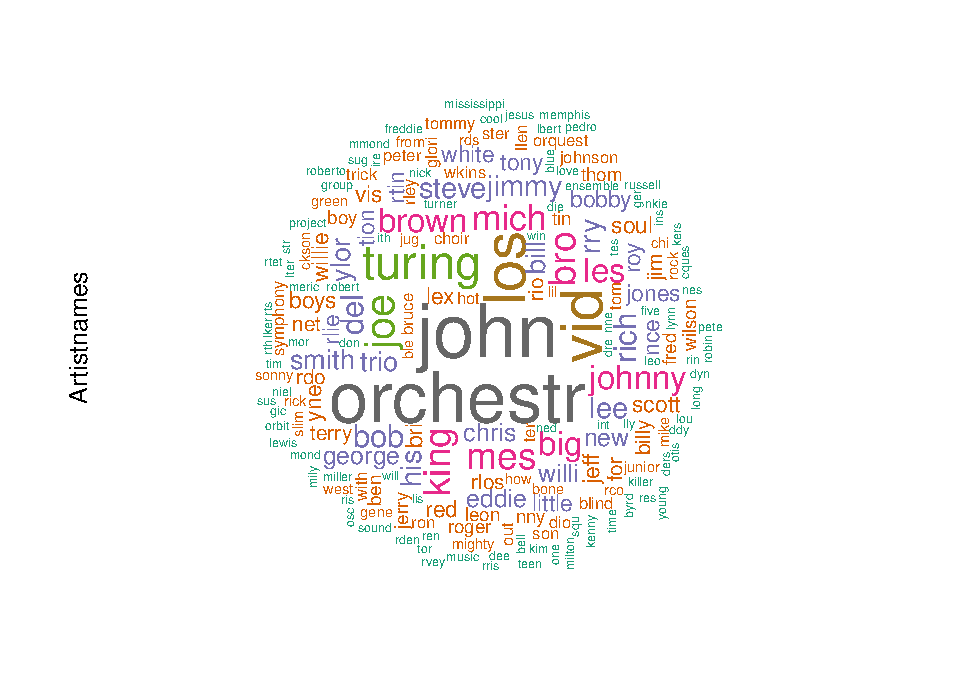
\includegraphics{Project2_files/figure-latex/wordclodArtist-1.pdf}

When looking at the word cloud above, one can see that the most common
artist names are either `orchestra' or `John'. Also there are some
spanish artist names containing words like `los'. This can be used to
gain a greater knowledge about the dataset. It becomes more clear that
artists do not only come from England, Europe or the US but also from
Spain or Latin America. One could get rid of the prepositions in all
languages the dataset contains. Thus the preposition `los' should alse
be wiped out. Some other names like `Joe' or `King' are also quite
commonly used. To make some more assumptions and to get a better
understanding of the word cloud, the actual frequencies of the very
frequent entries where provided in a table.

\begin{Shaded}
\begin{Highlighting}[]
\CommentTok{# show only head of frequency dataFrame}
\KeywordTok{head}\NormalTok{(d,}\DecValTok{8}\NormalTok{)}
\end{Highlighting}
\end{Shaded}

\begin{verbatim}
##              word freq
## john         john   41
## orchestr orchestr   38
## los           los   31
## vid           vid   31
## turing     turing   25
## joe           joe   21
## bro           bro   19
## king         king   19
\end{verbatim}

Together with this table and the word cloud one can gain a better
understanding of the distribution of the artist names in the given
dataset. Now it is interesting to get some more facts about the most
common name `John'. After a small research on the internet
{[}research{]} one can see, that John was one of the most common names
in the 1990's. To prove that this name occured mostly in the 1990's in
the dataset one can take a closer look on the data of respective years.

\begin{Shaded}
\begin{Highlighting}[]
\NormalTok{tracksPerYear}\OperatorTok{$}\NormalTok{artistName[tracksPerYear}\OperatorTok{$}\NormalTok{Year }\OperatorTok{>=}\StringTok{ }\DecValTok{1990} \OperatorTok{&}\StringTok{ }\NormalTok{tracksPerYear}\OperatorTok{$}\NormalTok{Year }\OperatorTok{<=}\StringTok{ }\DecValTok{2000}\NormalTok{]}
\end{Highlighting}
\end{Shaded}

\begin{verbatim}
##  [1] K's Choice            K's Choice            Kaija Koo            
##  [4] Kisha                 Lee Ritenour          Les Malpolis         
##  [7] Lisa Lynne            Los Amigos Invisibles Los Amigos Invisibles
## [10] Luciana Souza         M.A. Numminen         Mandi                
## [13] Martin Sexton         Martin Sexton         Mithotyn             
## [16] Mithotyn              Monster Magnet        Moonspell            
## [19] Mudhoney              Natural Elements      Nic Endo             
## [22] Old Man's Child       OutKast              
## 1149 Levels: !!! 2 Minutos 2-4 Grooves feat. Reki D. ... Zombina & The Skeletones
\end{verbatim}

After displaying the actual dataset and the entries of the artist names
between the years 1990 and 2000, the assumption made before should be
declined. However one can see another common word in the displayed
subset `Los'. This set needs to be more described and explored, because
the previous exploration does not provide a lot of information.

\subsection{Visualize songnames}\label{visualize-songnames}

Almost the same analysis was done on common song names. However the
common words in this case were not quite the same as in the script
before. The method we used to find common song names was to plot the
word cloud as an uncleaned version, containing all possible words. After
deciding which words do not have a proper meaning to the final statement
it was obvious to delete those words. Thus the cleaning with words like
`the',`version',`and',`from', `feat' and `album' created the following
word cloud.

\begin{Shaded}
\begin{Highlighting}[]
\NormalTok{docs <-}\StringTok{ }\KeywordTok{Corpus}\NormalTok{(}\KeywordTok{VectorSource}\NormalTok{(}\KeywordTok{as.character}\NormalTok{(tracks}\OperatorTok{$}\NormalTok{songName)))}

\CommentTok{# Convert the text to lower case}
\NormalTok{docs <-}\StringTok{ }\KeywordTok{tm_map}\NormalTok{(docs, }\KeywordTok{content_transformer}\NormalTok{(tolower))}

\NormalTok{others <-}\StringTok{ }\KeywordTok{c}\NormalTok{(}\StringTok{'the'}\NormalTok{,}\StringTok{'version'}\NormalTok{,}\StringTok{'and'}\NormalTok{,}\StringTok{'from'}\NormalTok{, }\StringTok{'feat'}\NormalTok{,}\StringTok{'album'}\NormalTok{)}
\NormalTok{toSpace <-}\StringTok{ }\KeywordTok{content_transformer}\NormalTok{(}\ControlFlowTok{function}\NormalTok{ (x , pattern ) }\KeywordTok{gsub}\NormalTok{(pattern, }\StringTok{" "}\NormalTok{, x))}
\ControlFlowTok{for}\NormalTok{ (i }\ControlFlowTok{in} \DecValTok{1}\OperatorTok{:}\KeywordTok{length}\NormalTok{(others))\{}
\NormalTok{docs <-}\StringTok{ }\KeywordTok{tm_map}\NormalTok{(docs, toSpace, others[i])}
\NormalTok{\}}

\NormalTok{dtm <-}\StringTok{ }\KeywordTok{TermDocumentMatrix}\NormalTok{(docs)}
\NormalTok{m <-}\StringTok{ }\KeywordTok{as.matrix}\NormalTok{(dtm)}
\NormalTok{v <-}\StringTok{ }\KeywordTok{sort}\NormalTok{(}\KeywordTok{rowSums}\NormalTok{(m),}\DataTypeTok{decreasing=}\OtherTok{TRUE}\NormalTok{)}
\NormalTok{d <-}\StringTok{ }\KeywordTok{data.frame}\NormalTok{(}\DataTypeTok{word =} \KeywordTok{names}\NormalTok{(v),}\DataTypeTok{freq=}\NormalTok{v)}

\KeywordTok{wordcloud}\NormalTok{(}\DataTypeTok{words =}\NormalTok{ d}\OperatorTok{$}\NormalTok{word, }\DataTypeTok{freq =}\NormalTok{ d}\OperatorTok{$}\NormalTok{freq, }\DataTypeTok{min.freq =} \DecValTok{1}\NormalTok{, }
          \DataTypeTok{max.words=}\DecValTok{100}\NormalTok{, }\DataTypeTok{random.order=}\OtherTok{FALSE}\NormalTok{, }\DataTypeTok{rot.per=}\FloatTok{0.35}\NormalTok{, }\DataTypeTok{colors=}\KeywordTok{brewer.pal}\NormalTok{(}\DecValTok{8}\NormalTok{, }\StringTok{"Dark2"}\NormalTok{))}
\KeywordTok{mtext}\NormalTok{(}\StringTok{'Songnames'}\NormalTok{, }\DataTypeTok{side =} \DecValTok{3}\NormalTok{, }\DataTypeTok{line =} \DecValTok{0}\NormalTok{, }\DataTypeTok{adj =} \FloatTok{0.5}\NormalTok{) }\CommentTok{# title}
\end{Highlighting}
\end{Shaded}

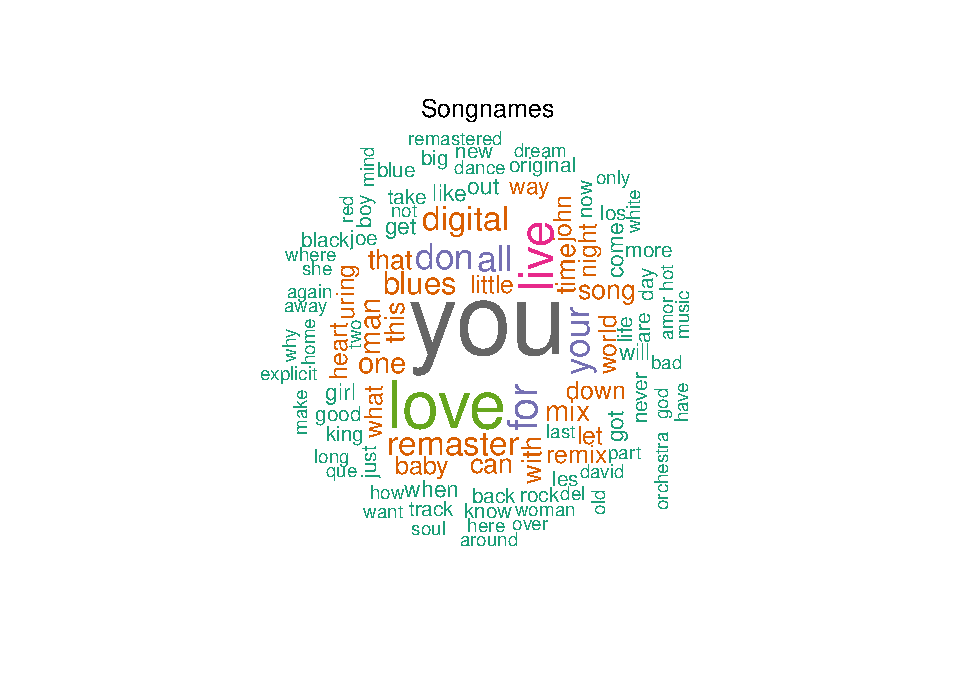
\includegraphics{Project2_files/figure-latex/wordcloudSongname-1.pdf}

Looking at the result one can see the frequently words `you' and `love'.
Interpreting this result, it is obvious that this dataset consists of
song names that are more likely to address love and the counterpart of a
human, you. A general assumption could be, that there are more songs
addressing Love, the counterpart of someone and the life, following
topics about the world or travelling for example. However this
assumption can not be completely proven since this dataset does not
represent all the song names in the world.

Also by looking at the following table, one can have a better and more
detailed information about the distribution of the song names.

\begin{Shaded}
\begin{Highlighting}[]
\KeywordTok{head}\NormalTok{(d,}\DecValTok{7}\NormalTok{)}
\end{Highlighting}
\end{Shaded}

\begin{verbatim}
##      word freq
## you   you  540
## love love  332
## live live  216
## for   for  185
## all   all  144
## your your  143
## don   don  137
\end{verbatim}

\subsection{Visualize artist
locations}\label{visualize-artist-locations}

Since it is clear that the dataset not only contains artists from
England or Europe or the US, it would be nice to have a proper plot of
the world together with the location of the artists. This can be
achieved through the package `maps' \footnote{\url{https://cran.r-project.org/web/packages/maps/maps.pdf}
  page view {[}25.06.18{]}}. This package provides not only a method to
draw a map by accessing it through a word like world but also by giving
this method a border by longitude and latitude to get a closer look on
different parts of it. It is easy to use and draw complex maps as well
as set some points on the map. The world map below shows all artists
with their respective locations. Unfortinately the dataset does not
provide a location for each artist, but nevertheless it creates a good
overview.

\begin{Shaded}
\begin{Highlighting}[]
\KeywordTok{library}\NormalTok{(maps)}

\CommentTok{# parse the lat and lon values of given set }
\NormalTok{lon <-}\StringTok{ }\KeywordTok{as.double}\NormalTok{(}\KeywordTok{as.character}\NormalTok{(location}\OperatorTok{$}\NormalTok{lon))}
\NormalTok{lat <-}\StringTok{ }\KeywordTok{as.double}\NormalTok{(}\KeywordTok{as.character}\NormalTok{(location}\OperatorTok{$}\NormalTok{lat))}

\CommentTok{# delete all NaN}
\NormalTok{lon <-}\StringTok{ }\NormalTok{lon[}\OperatorTok{!}\KeywordTok{is.na}\NormalTok{(lon)]}
\NormalTok{lat <-}\StringTok{ }\NormalTok{lat[}\OperatorTok{!}\KeywordTok{is.na}\NormalTok{(lat)]}

\NormalTok{coordinates <-}\StringTok{ }\KeywordTok{as.data.frame}\NormalTok{(}\KeywordTok{cbind}\NormalTok{(lon, lat))}

\CommentTok{# world map }
\KeywordTok{map}\NormalTok{(}\StringTok{'world'}\NormalTok{,}\KeywordTok{c}\NormalTok{(}\StringTok{'.'}\NormalTok{), }\DataTypeTok{col =} \StringTok{"grey80"}\NormalTok{, }\DataTypeTok{fill =} \OtherTok{TRUE}\NormalTok{, }\DataTypeTok{border =} \StringTok{"grey40"}\NormalTok{) }
\KeywordTok{points}\NormalTok{(coordinates}\OperatorTok{$}\NormalTok{lon, coordinates}\OperatorTok{$}\NormalTok{lat, }\DataTypeTok{col =} \StringTok{"red"}\NormalTok{, }\DataTypeTok{cex =}\NormalTok{ .}\DecValTok{1}\NormalTok{)}
\end{Highlighting}
\end{Shaded}

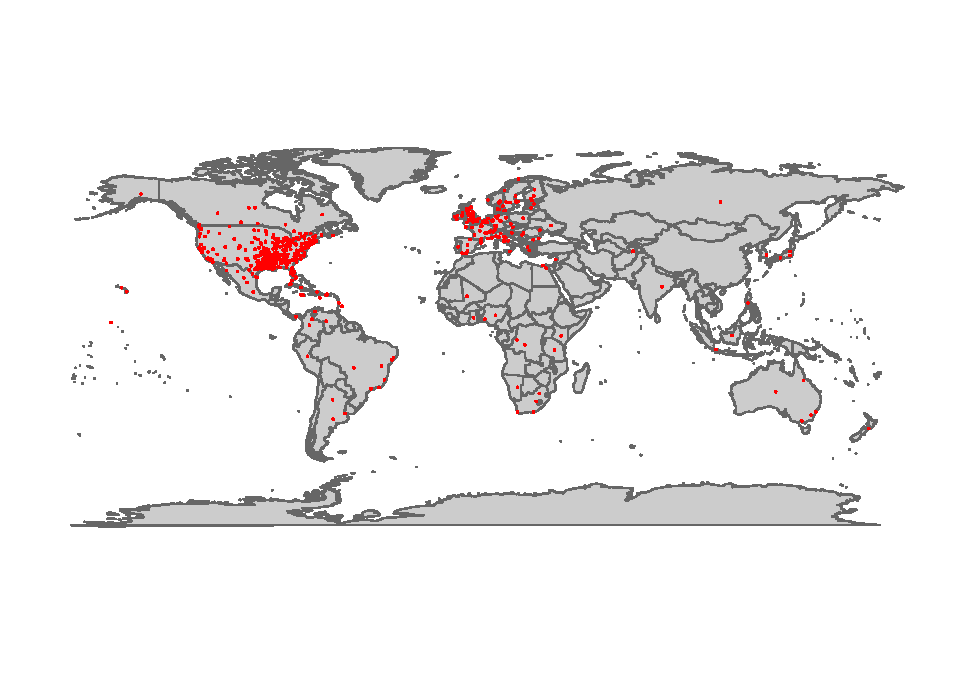
\includegraphics{Project2_files/figure-latex/worldmapArtist -1.pdf}

The assumptions about the artists made beforehand are completely right.
The data not only consist of European and English speaking artist but
also of people from around the world. Mostly the artists come from the
US and Europe, some even from Russia or Australia or as assumed before
from Latin America. By looking at the song names it is hard to tell
wether the artist is from Australia or the US. With this representation
one can have a better understanding of the dataset and finally clarify
the unclarified.

An even closer look on Europe is provided by the map below. Due to the
blurred representation of Europe in the worldmap, this map was created.
Especially because of the actual location of the author and the location
of the university this representation was chosen.

\begin{Shaded}
\begin{Highlighting}[]
\CommentTok{# europe map}
\KeywordTok{map}\NormalTok{(}\DataTypeTok{col =} \StringTok{"grey80"}\NormalTok{, }\DataTypeTok{border =} \StringTok{"grey40"}\NormalTok{, }\DataTypeTok{fill =} \OtherTok{TRUE}\NormalTok{,}
  \DataTypeTok{xlim =} \KeywordTok{c}\NormalTok{(}\OperatorTok{-}\DecValTok{25}\NormalTok{, }\DecValTok{45}\NormalTok{), }\DataTypeTok{ylim =} \KeywordTok{c}\NormalTok{(}\DecValTok{36}\NormalTok{, }\DecValTok{70}\NormalTok{), }\DataTypeTok{mar =} \KeywordTok{rep}\NormalTok{(}\FloatTok{0.1}\NormalTok{, }\DecValTok{4}\NormalTok{))}
\KeywordTok{points}\NormalTok{(coordinates}\OperatorTok{$}\NormalTok{lon, coordinates}\OperatorTok{$}\NormalTok{lat, }\DataTypeTok{col =} \StringTok{"red"}\NormalTok{, }\DataTypeTok{cex =}\NormalTok{ .}\DecValTok{3}\NormalTok{)}
\end{Highlighting}
\end{Shaded}

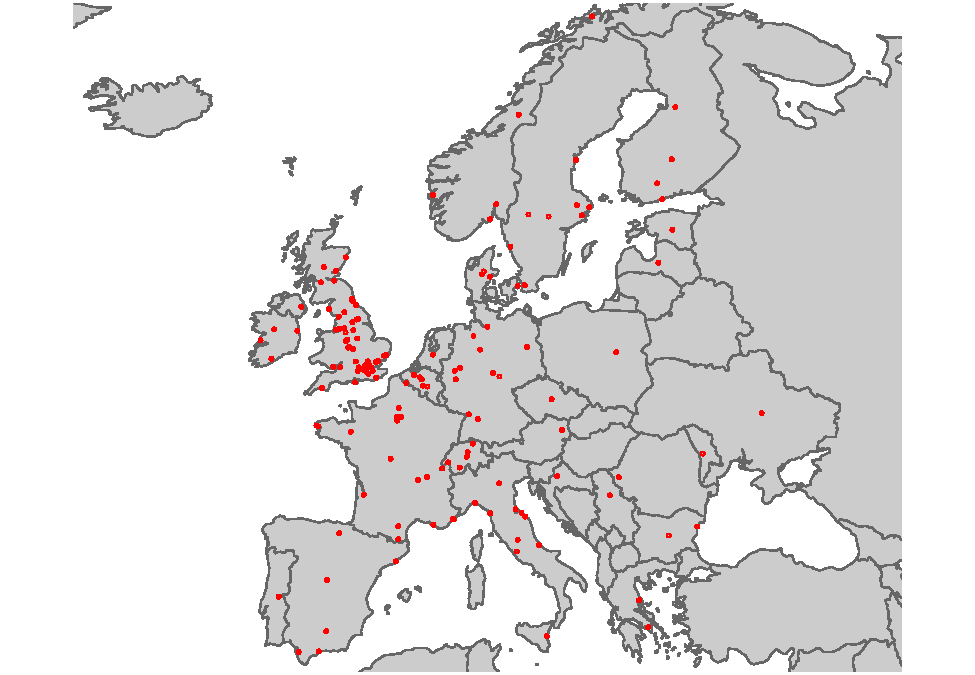
\includegraphics{Project2_files/figure-latex/europemapArtist-1.pdf}

\section{Analyse choosen Songs}\label{analyse-choosen-songs}

As mentioned before the goal we set ourselves for this task, was to find
similarities of favorite songs and to compare those to a recommendation
made by Spotify. To achive this, one should be able to read in the
provided data in HDF5 Format. Therefore, it is required to load the
package `rhdf5' \footnote{load \textless{}
  source(``\url{http://bioconductor.org/biocLite.R}'');
  biocLite(``rhdf5'') \textgreater{}} that helps accessing the data
files and get the information to analize it. The chosen data is a
preference of a person of our group. The songs he had chosen are ordered
as followed:

\begin{itemize}
\item
  Beynonce Single Ladies TrackID: TRAPZTV128F92CAA4E 
\item
  Justin Timberlake What Goes Around Comes Around TrackID:
  TRANNZZ128F92C22F7 
\item
  Kanye West / Lupe Fiasco Touch The Sky TrackID: TRAQZQX128F931338F 
\item
  Madonna Jump TrackID: TRALONM128EF35A199 
\item
  B.o.B Nothin on You feat Bruno Mars TrackID: TRAWBHE12903CBC4CB 
\end{itemize}

Taking the TrackID that functions also as the file name, one should
first find out the right paths to the preferred files to access them.
After creating the right path one should be able to access the data
through some methods. As described below there are two methods to read
in data. The first one is to access the groups with method h5ls() and
the second one to access the data in those groups with method h5read().
One can see a slice of an output for h5ls() underneath.

\begin{Shaded}
\begin{Highlighting}[]
\KeywordTok{library}\NormalTok{(tcltk) }\CommentTok{# for interactive file choosing}
\KeywordTok{library}\NormalTok{(rhdf5) }\CommentTok{# required for H5 files}

\CommentTok{# dynamic path }
\CommentTok{# important to have the MIllion Song Data subset downloaded}
\CommentTok{# pathToSet <- tk_choose.dir(default = "", caption = "Select directory")}

\CommentTok{# set a hardcoded Path to the MillionSongSubset}
\NormalTok{pathToSet =}\StringTok{ '/Users/Kostja/Desktop/Master/Sem 2 (18 SoSe)/Data Visualization/Tasks/MillionSongSubset'}

\CommentTok{# create array with found Ids in beforehand containing prefered songs}
\NormalTok{TrackIDs <-}\StringTok{ }\KeywordTok{array}\NormalTok{(}\KeywordTok{c}\NormalTok{(}\StringTok{'TRAPZTV128F92CAA4E'}\NormalTok{,}\StringTok{'TRANNZZ128F92C22F7'}\NormalTok{,}\StringTok{'TRAQZQX128F931338F'}\NormalTok{,}\StringTok{'TRALONM128EF35A199'}\NormalTok{,}\StringTok{'TRAWBHE12903CBC4CB'}\NormalTok{))}

\CommentTok{# find automaticaly all paths with names of trackIDs}
\NormalTok{SubPaths <-}\StringTok{ }\KeywordTok{lapply}\NormalTok{(TrackIDs,find.path <-}\StringTok{ }\ControlFlowTok{function}\NormalTok{(x)\{}
  \KeywordTok{list.files}\NormalTok{(pathToSet, x, }\DataTypeTok{recursive=}\OtherTok{TRUE}\NormalTok{, }\DataTypeTok{full.names=}\OtherTok{TRUE}\NormalTok{, }\DataTypeTok{include.dirs=}\OtherTok{TRUE}\NormalTok{)}
\NormalTok{\})}

\CommentTok{# beautify the dataset }
\NormalTok{SubPaths <-}\StringTok{ }\KeywordTok{data.frame}\NormalTok{(}\DataTypeTok{SubPaths =} \KeywordTok{t}\NormalTok{(}\KeywordTok{unlist}\NormalTok{(SubPaths)))}
\KeywordTok{names}\NormalTok{(SubPaths) <-}\StringTok{ }\KeywordTok{c}\NormalTok{(}\StringTok{'beyonce'}\NormalTok{, }\StringTok{'justin'}\NormalTok{, }\StringTok{'kanye'}\NormalTok{, }\StringTok{'madonna'}\NormalTok{, }\StringTok{'bruno'}\NormalTok{)}

\CommentTok{# read the H5 files and create a readable output}
\NormalTok{artist <-}\StringTok{ }\KeywordTok{lapply}\NormalTok{(SubPaths, }\ControlFlowTok{function}\NormalTok{(x)\{}
  \KeywordTok{h5ls}\NormalTok{(}\KeywordTok{toString}\NormalTok{(x))}
\NormalTok{\})}

\KeywordTok{head}\NormalTok{(artist}\OperatorTok{$}\NormalTok{beyonce,}\DecValTok{23}\NormalTok{)}
\end{Highlighting}
\end{Shaded}

\begin{verbatim}
##        group                       name       otype   dclass       dim
## 0          /                   analysis   H5I_GROUP                   
## 1  /analysis            bars_confidence H5I_DATASET    FLOAT       639
## 2  /analysis                 bars_start H5I_DATASET    FLOAT       639
## 3  /analysis           beats_confidence H5I_DATASET    FLOAT       639
## 4  /analysis                beats_start H5I_DATASET    FLOAT       639
## 5  /analysis        sections_confidence H5I_DATASET    FLOAT        13
## 6  /analysis             sections_start H5I_DATASET    FLOAT        13
## 7  /analysis        segments_confidence H5I_DATASET    FLOAT      1818
## 8  /analysis      segments_loudness_max H5I_DATASET    FLOAT      1818
## 9  /analysis segments_loudness_max_time H5I_DATASET    FLOAT      1818
## 10 /analysis    segments_loudness_start H5I_DATASET    FLOAT      1818
## 11 /analysis           segments_pitches H5I_DATASET    FLOAT 12 x 1818
## 12 /analysis             segments_start H5I_DATASET    FLOAT      1818
## 13 /analysis            segments_timbre H5I_DATASET    FLOAT 12 x 1818
## 14 /analysis                      songs H5I_DATASET COMPOUND         1
## 15 /analysis          tatums_confidence H5I_DATASET    FLOAT      1278
## 16 /analysis               tatums_start H5I_DATASET    FLOAT      1278
## 17         /                   metadata   H5I_GROUP                   
## 18 /metadata               artist_terms H5I_DATASET   STRING        28
## 19 /metadata          artist_terms_freq H5I_DATASET    FLOAT        28
## 20 /metadata        artist_terms_weight H5I_DATASET    FLOAT        28
## 21 /metadata            similar_artists H5I_DATASET   STRING       100
## 22 /metadata                      songs H5I_DATASET COMPOUND         1
\end{verbatim}

This snippet shows that there are different groups and even different
subgroups one can access through h5read(). An example of the final data
of Beyonce's song of group analysis and metadata can be seen underneath.

\begin{Shaded}
\begin{Highlighting}[]
\NormalTok{Analyze_song <-}\StringTok{ }\KeywordTok{apply}\NormalTok{(SubPaths,}\DecValTok{2}\NormalTok{,}\ControlFlowTok{function}\NormalTok{(x)\{}
  \KeywordTok{h5read}\NormalTok{(x,}\StringTok{"/analysis/songs"}\NormalTok{)}
\NormalTok{\})}
\NormalTok{Analyze_song <-}\StringTok{ }\KeywordTok{do.call}\NormalTok{(rbind, Analyze_song)}

\NormalTok{Meta_song <-}\StringTok{ }\KeywordTok{apply}\NormalTok{(SubPaths,}\DecValTok{2}\NormalTok{,}\ControlFlowTok{function}\NormalTok{(x)\{}
  \KeywordTok{h5read}\NormalTok{(x,}\StringTok{"/metadata/songs"}\NormalTok{)}
\NormalTok{\})}
\NormalTok{Meta_song <-}\StringTok{ }\KeywordTok{do.call}\NormalTok{(rbind, Meta_song)}

\CommentTok{# will be used in PCA for ploting timbre}
\NormalTok{track_timbre <-}\StringTok{ }\KeywordTok{apply}\NormalTok{(SubPaths,}\DecValTok{2}\NormalTok{,}\ControlFlowTok{function}\NormalTok{(x)\{}
  \KeywordTok{h5read}\NormalTok{(x,}\StringTok{"/analysis/segments_timbre"}\NormalTok{)}
\NormalTok{\})}

\CommentTok{# will be used in PCA for ploting pitch}
\NormalTok{track_pitch <-}\StringTok{ }\KeywordTok{apply}\NormalTok{(SubPaths,}\DecValTok{2}\NormalTok{,}\ControlFlowTok{function}\NormalTok{(x)\{}
  \KeywordTok{h5read}\NormalTok{(x,}\StringTok{"/analysis/segments_pitches"}\NormalTok{)}
\NormalTok{\})}
\CommentTok{# example to show and see the entries of subgroups }
\KeywordTok{t}\NormalTok{(Analyze_song[}\StringTok{'beyonce'}\NormalTok{,])}
\end{Highlighting}
\end{Shaded}

\begin{verbatim}
##                                beyonce                           
## analysis_sample_rate           "22050"                           
## audio_md5                      "dea6eb2198d4e2a93d5c0ae5df27820b"
## danceability                   "0"                               
## duration                       "466.0502"                        
## end_of_fade_in                 "0.293"                           
## energy                         "0"                               
## idx_bars_confidence            "0"                               
## idx_bars_start                 "0"                               
## idx_beats_confidence           "0"                               
## idx_beats_start                "0"                               
## idx_sections_confidence        "0"                               
## idx_sections_start             "0"                               
## idx_segments_confidence        "0"                               
## idx_segments_loudness_max      "0"                               
## idx_segments_loudness_max_time "0"                               
## idx_segments_loudness_start    "0"                               
## idx_segments_pitches           "0"                               
## idx_segments_start             "0"                               
## idx_segments_timbre            "0"                               
## idx_tatums_confidence          "0"                               
## idx_tatums_start               "0"                               
## key                            "11"                              
## key_confidence                 "0.847"                           
## loudness                       "-6.593"                          
## mode                           "0"                               
## mode_confidence                "0.58"                            
## start_of_fade_out              "454.246"                         
## tempo                          "84.1"                            
## time_signature                 "1"                               
## time_signature_confidence      "1"                               
## track_id                       "TRAPZTV128F92CAA4E"
\end{verbatim}

\begin{Shaded}
\begin{Highlighting}[]
\KeywordTok{t}\NormalTok{(Meta_song[}\StringTok{'beyonce'}\NormalTok{,])}
\end{Highlighting}
\end{Shaded}

\begin{verbatim}
##                     beyonce                                           
## analyzer_version    ""                                                
## artist_7digitalid   "21453"                                           
## artist_familiarity  "0.8894607"                                       
## artist_hotttnesss   "0.6194314"                                       
## artist_id           "AR65K7A1187FB4DAA4"                              
## artist_latitude     NA                                                
## artist_location     ""                                                
## artist_longitude    NA                                                
## artist_mbid         "183105b5-3e68-4748-9086-2c1c11bf7a3d"            
## artist_name         "Beyoncé"                                         
## artist_playmeid     "193"                                             
## genre               ""                                                
## idx_artist_terms    "0"                                               
## idx_similar_artists "0"                                               
## release             "Single Ladies (Put A Ring On It) - Dance Remixes"
## release_7digitalid  "372352"                                          
## song_hotttnesss     NA                                                
## song_id             "SOFQBMN12A8C1428AD"                              
## title               "Single Ladies (Put A Ring On It)"                
## track_7digitalid    "4143185"
\end{verbatim}

Both tables will be used and combined on different variables. What also
draws attention is the sparse vectors in the table above. Obviously one
should get rid of those and just use the other variables for comparison.

First, one has to decide which variables one should take and what the
meaning of those is. Second, it is important to decide which of those
variables is comparable and where the similarities between the songs
are. Hence, one needs to make further detailed analysis on the given
data. Finally, one should be able to predict any given song if it fits
the calculated results and the predicted song would be recommended to
that person.

\subsection{Data discription}\label{data-discription}

By looking at the data without any knowledge in beforehand, one should
understand each an every variable. Since this has been done already, we
will focus on the chosen variables and describe those. Variables:

\begin{itemize}
\item
  Tempo: Indicates the speed of a beat and is also known as Beats per
  Minute (BPM). It is derived directly from avarage beat duration
  \footnote{\url{http://docs.echonest.com.s3-website-us-east-1.amazonaws.com/_static/AnalyzeDocumentation.pdf}
    page view {[}01.07.18{]}}. This is a basic unit of time in music.
  Now it is important to understand what exactly a beat is. To simplify
  the statement it is the rythm when a listener would tap his toe to a
  music sequence \footnote{\url{https://en.wikipedia.org/wiki/Beat_(music)}
    page view {[}04.07.18{]}}. BPM Examples are 60 BPM would be a beat
  per second and 120 BPM would be 2 beats per second \footnote{\url{https://www.rhythm-in-music.com/introduction-beat-and-tempo.html}
    page view {[}04.07.18{]}}. 
\item
  Loudness: This indicates the overall loudness of a track in decibels
  (dB) and is avaraged across a track in this dataset. The loudness is
  correlated with the physical strength in the given dataset the
  loudness is averaged across a track \footnote{\url{http://docs.echonest.com.s3-website-us-east-1.amazonaws.com/_static/AnalyzeDocumentation.pdf}
    page view {[}01.07.18{]}}. 
\item
  Mode: In the theory of Western music, a mode is a type of musical
  scale coupled with a set of characteristic melodic behaviors.
  \footnote{\url{https://en.wikipedia.org/wiki/Mode_(music)} page view
    {[}01.07.18{]}}. To simplify this statement a mode could be seen as
  the vocabulary of a melody. It specifies which notes can be used and
  indicates which have special importance \footnote{\url{https://www.britannica.com/art/mode-music}
    page view {[}04.07.18{]}}. Mostly major notes sound happy and minor
  notes do not \footnote{\url{https://insights.spotify.com/it/2015/05/06/most-popular-keys-on-spotify/}
    page view {[}04.07.18{]}} 
\item
  Key: The key of a song refers to a tonal center of it and will also
  determine what notes and chords a song should use \footnote{\url{https://insights.spotify.com/it/2015/05/06/most-popular-keys-on-spotify/}
    page view {[}04.07.18{]}}. The key also identifies the tonic triad,
  the chord, major or minor, which represents the final point of rest of
  a piece \footnote{\url{http://docs.echonest.com.s3-website-us-east-1.amazonaws.com/_static/AnalyzeDocumentation.pdf}
    page view {[}01.07.18{]}}. An example of a key could be C C\# D E F
  G etc.
\item
  Time Signature: The time signature, also known as meter signature, is
  a notational convention to specify how many beats are in each bar
  \footnote{\url{http://docs.echonest.com.s3-website-us-east-1.amazonaws.com/_static/AnalyzeDocumentation.pdf}
    page view {[}01.07.18{]}}. So now it is important to understand what
  exactly a bar is. A bar (or measure) is a segment of time
  corresponding to a specific number of beats in which each beat is
  represented by a particular note value and the boundaries of the bar
  are indicated by vertical bar lines \footnote{\url{https://en.wikipedia.org/wiki/Bar_(music)}
    page view {[}04.07.18{]}}.
\end{itemize}

\begin{figure}
\centering
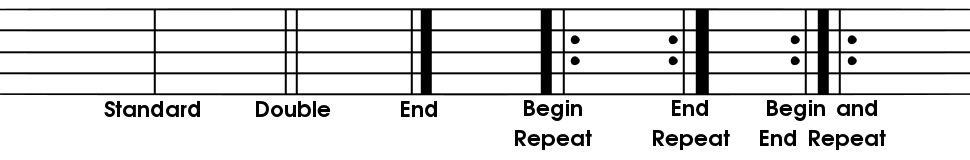
\includegraphics{./picturesDocu/970px-Barlines.svg.png}
\caption{\url{https://en.wikipedia.org/wiki/Bar_(music)}}
\end{figure}

As can be seen in the picture above, a bar could be simplified through a
vertical line in music notes.

\begin{itemize}
\tightlist
\item
  Segment Pitch: A pitch is a position of a single sound in the complete
  range of sound. Sounds are higher or lower in pitch according to the
  frequency of vibration of the sound waves producing them \footnote{\url{https://www.britannica.com/art/pitch-music}
    page view {[}04.07.18{]}}. For a better understanding one should
  take a look on the further picture. But also one should have a better
  understanding of a segment. A segment is a set of sound entities,
  typically under a second, each relatively uniform in timbre and
  harmony. Segments are characterized by their perceptual onsets and
  duration in seconds, loudness (dB), pitch and timbral content
  \footnote{\url{http://docs.echonest.com.s3-website-us-east-1.amazonaws.com/_static/AnalyzeDocumentation.pdf}
    page view {[}01.07.18{]}}.
\end{itemize}

\begin{figure}
\centering
\includegraphics{./picturesDocu/pitch.gif}
\caption{\url{https://nuartapp.wordpress.com/2014/07/20/elements-of-music/}}
\end{figure}

 - Segment Timbre: Timbre is the quality of a musical note or sound that
distinguishes different types of musical instruments, or voices. It is a
complex notation also referred to as sound color, texture, or tone
quality \footnote{\url{http://docs.echonest.com.s3-website-us-east-1.amazonaws.com/_static/AnalyzeDocumentation.pdf}
  page view {[}01.07.18{]}}. The Echo Nest Analyzer's timbre feature is
a vector that includes 12 unbounded values roughly centered around 0.
This is represented as 12-dimensional vectors that are the principal
components of Mel-frequency cepstral co- efficients (MFCCs). They
represent the power spectrum of sound, and are derived from Fourier
analysis and further processing \footnote{\url{http://www.ee.columbia.edu/~dliang/files/FINAL.pdf}
  page view {[}06.07.18{]}}. For completeness however, the first
dimension represents the average loudness of the segment; second
emphasizes brightness; third is more closely correlated to the flatness
of a sound; fourth to sounds with a stronger attack; etc \footnote{\url{http://docs.echonest.com.s3-website-us-east-1.amazonaws.com/_static/AnalyzeDocumentation.pdf}
  page view {[}01.07.18{]}}.

\begin{itemize}
\tightlist
\item
  artist familiarity: Familiarity is an indication of how well known the
  artist is in 2010. \footnote{\url{https://musicmachinery.com/2009/05/25/artist-similarity-familiarity-and-hotness/}
    page view {[}06.07.18{]}}
\item
  artist hotness: Hotness (which is spelled as the zoolanderish
  `hotttnesss') is an indication of how much buzz the artist is getting
  in 2010. \footnote{\url{https://musicmachinery.com/2009/05/25/artist-similarity-familiarity-and-hotness/}
    page view {[}06.07.18{]}}
\end{itemize}

\subsubsection{Describing relations between the
variables}\label{describing-relations-between-the-variables}

With all the provided information in the section above, one can derive a
more specific representation of all the variables as well as a
relationship between them. As can be seen below and also written in
various articles, especially on Spotify, emotion is a very important
characteristic of music. Most people listen to music when they are sad
or happy or try to project their feelings on to it. Therefore, emotion
does have specific role when talking about music \footnote{\url{https://insights.spotify.com/it/2015/05/06/most-popular-keys-on-spotify/}
  page view {[}04.07.18{]}}. In addition to that there is also the genre
of a song and even an artist, that depends on other variables. It is
also a very important characteristic that can predict a listeners taste
of music. Most people tend to listen to one or two particular genres.
For sure there are more overall variables like emotion and genre, but
for now we limit ourself to only those two.

\begin{figure}
\centering
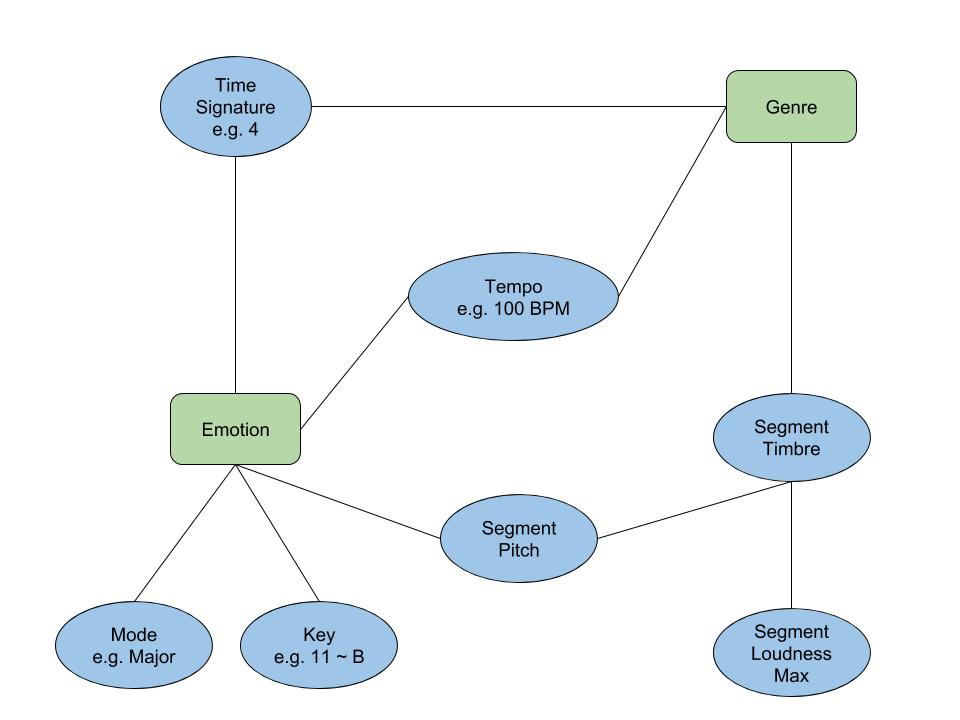
\includegraphics{./picturesDocu/Variable.jpg}
\caption{Self created picture for the relationship between the
variables}
\end{figure}

As provided by the image above, that was created by ourselves, the
variables tend to describe the overall variables. Our research on the
variables, led to this picture. Here one can see properly that the
relationship for emotion does of course consist of all the variables,
since the whole package of information does lead towards a proper and
confident answer, but also it is highly dependent on the key and the
mode. As mentioned in the section `Data discription' especially the
mode, mostly tends to describe either if the song is a happy one or not.
Here one can see that key is a reliable source for measuring the emotion
as well, since it correlates with the mode. Also the pitch is
corresponding to one of the 12 keys and therefore, is a reliable source
for emotions too.

\paragraph{ab hier muss korriegiert werden und anschließend diese
Section
weg}\label{ab-hier-muss-korriegiert-werden-und-anschlieend-diese-section-weg}

As can be seen in this image too, the tempo does provide as well the
emotion as well as the genre. Typically a higher tempo describes a more
happy song and a genre like pop or techno or something similar. Also the
time signature, which does rely on beat as well as the tempo, could
describe an emotion or a genre. Sigment Timbre however provides more a
genre then an Emotion because it relies more on different types of
musical instruments and some musical instruments do tend to be used in a
particular genre like a guitar is common to use in Latin American songs.
But together with the pitch, which does use the distribution of the
keys, the timbre could be used to determine the emotion too. All of the
preposition can be seen in the image above. The background information
does come from a research our group atended and can be reproduced with
the sources and footnotes in the very last section.

\subsection{Finding similarities}\label{finding-similarities}

\subsubsection{General comparison}\label{general-comparison}

Since there is enough information about the choosen variables one should
attend to get a better overview about the songs. Hence our group chosed
the followed variables to compare the songs.

\begin{itemize}
\tightlist
\item
  Loudness
\item
  Tempo
\item
  Mode
\item
  Key
\end{itemize}

We created a radarplot using the package `fmsb' \footnote{\url{https://cran.r-project.org/web/packages/fmsb/fmsb.pdf}
  page view {[}05.07.18{]}}. This package is mostly used for Medical and
Health Analysis in R, but can also be used for this purposes to
radarplot the characteristics of our data. Together with the method
`radarchart' one can plot a radar that creates a very good overview of
the characteristics. In the following Plot one can see some similarities
of the choosen songs.

\begin{Shaded}
\begin{Highlighting}[]
\KeywordTok{library}\NormalTok{(fmsb) }\CommentTok{# for radar charts}

\CommentTok{# function takes a dataframe and concatenates it}
\NormalTok{radarFrame <-}\StringTok{ }\ControlFlowTok{function}\NormalTok{(df2)\{}
\NormalTok{  matrix <-}\StringTok{ }\KeywordTok{cbind}\NormalTok{(}\StringTok{'loudness'}\NormalTok{ =}\StringTok{ }\NormalTok{df2}\OperatorTok{$}\NormalTok{loudness,}\StringTok{'tempo'}\NormalTok{=}\StringTok{ }\NormalTok{df2}\OperatorTok{$}\NormalTok{tempo, }\StringTok{'mode'}\NormalTok{ =}\StringTok{ }\NormalTok{df2}\OperatorTok{$}\NormalTok{mode, }\StringTok{'key'}\NormalTok{ =}\StringTok{ }\NormalTok{df2}\OperatorTok{$}\NormalTok{key) }
  \KeywordTok{rownames}\NormalTok{(matrix) <-}\StringTok{ }\KeywordTok{rownames}\NormalTok{(df2)}
\NormalTok{  matrix <-}\StringTok{ }\KeywordTok{data.frame}\NormalTok{(matrix)}
\NormalTok{\}}

\CommentTok{# creates a ArtistNameString out of dataframe information}
\NormalTok{namesLegend <-}\StringTok{ }\KeywordTok{paste}\NormalTok{(Meta_song}\OperatorTok{$}\NormalTok{artist_name,Meta_song}\OperatorTok{$}\NormalTok{title)}

\CommentTok{# plots the radar, function wants to have a dataframe with the data to plot }
\CommentTok{# artistnames for the legend as well as the optional coordinates where to plot the legend}
\NormalTok{radar <-}\StringTok{ }\ControlFlowTok{function}\NormalTok{(df, }\DataTypeTok{namesLeg =}\NormalTok{ namesLegend, }\DataTypeTok{x =} \OperatorTok{-}\FloatTok{2.8}\NormalTok{ , }\DataTypeTok{y=} \OperatorTok{-}\FloatTok{1.1}\NormalTok{)\{}
\NormalTok{  transparency <-}\StringTok{ }\KeywordTok{adjustcolor}\NormalTok{(}\DecValTok{1}\OperatorTok{:}\KeywordTok{dim}\NormalTok{(df)[}\DecValTok{1}\NormalTok{], }\DataTypeTok{alpha.f =} \FloatTok{0.2}\NormalTok{)}
  \CommentTok{# Custom the radarChart !}
  \KeywordTok{radarchart}\NormalTok{( df  , }\DataTypeTok{axistype=}\DecValTok{1}\NormalTok{ , }\DataTypeTok{maxmin =} \OtherTok{FALSE}\NormalTok{,}
    \CommentTok{#custom polygon}
    \DataTypeTok{pcol=}\DecValTok{1}\OperatorTok{:}\KeywordTok{dim}\NormalTok{(df)[}\DecValTok{1}\NormalTok{], }\DataTypeTok{plwd=}\DecValTok{1}\NormalTok{ , }\DataTypeTok{pfcol =}\NormalTok{ transparency ,}
    \CommentTok{#custom the grid}
    \DataTypeTok{cglcol=}\StringTok{"grey"}\NormalTok{, }\DataTypeTok{cglty=}\DecValTok{1}\NormalTok{, }\DataTypeTok{axislabcol=}\OtherTok{FALSE}\NormalTok{ ,}
    \CommentTok{#custom labels}
    \DataTypeTok{vlcex=}\FloatTok{0.8}
\NormalTok{    )}
  \KeywordTok{par}\NormalTok{(}\DataTypeTok{xpd=}\OtherTok{TRUE}\NormalTok{) }\CommentTok{# legend outside the plot }
\KeywordTok{legend}\NormalTok{(x,y, }\DataTypeTok{legend =}\NormalTok{ namesLeg, }\DataTypeTok{bty =} \StringTok{"n"}\NormalTok{, }\DataTypeTok{pch=}\DecValTok{20}\NormalTok{ , }\DataTypeTok{col=}\DecValTok{1}\OperatorTok{:}\KeywordTok{dim}\NormalTok{(df)[}\DecValTok{1}\NormalTok{] , }\DataTypeTok{cex=}\FloatTok{0.8}\NormalTok{, }\DataTypeTok{pt.cex=}\DecValTok{2}\NormalTok{)}
\NormalTok{\}}

\CommentTok{#create Dataframe suited for radar}
\NormalTok{data <-}\StringTok{ }\KeywordTok{radarFrame}\NormalTok{(Analyze_song)}

\CommentTok{# plot dataframe}
\KeywordTok{radar}\NormalTok{(data)}
\end{Highlighting}
\end{Shaded}

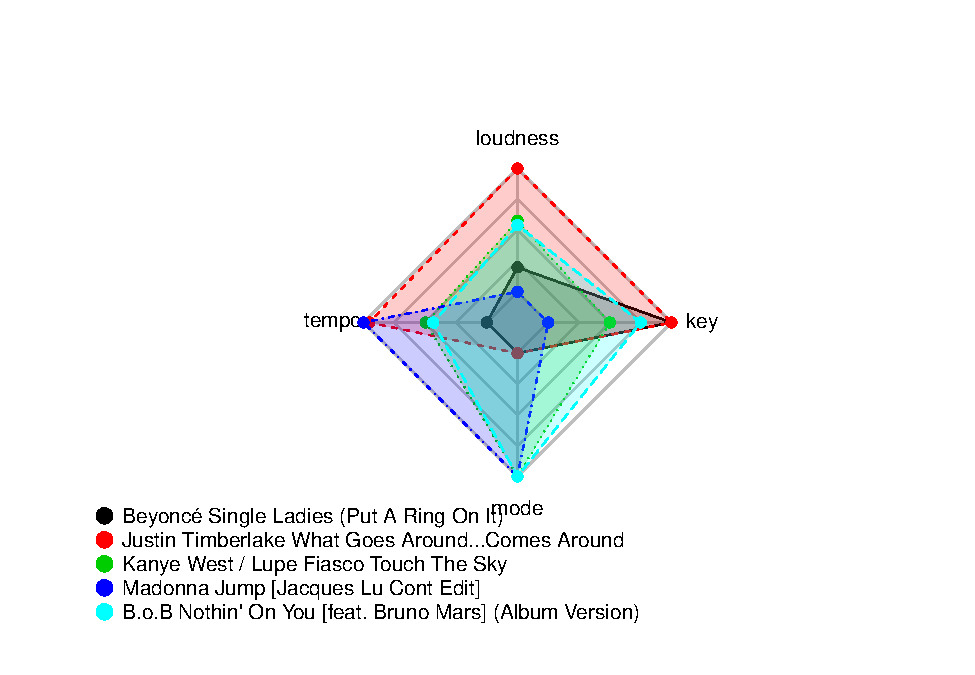
\includegraphics{Project2_files/figure-latex/crateRadar-1.pdf}

Looking at the plotted characteristics one can not see a real dependency
or even a realy good pattern. Mostly because the songs tend to be
similar, since a listener prefers them, but not in all ploted variables.
One could assume that key and tenpo tend to build clusters. Hence this
variables will be taken for a closer look. Nevertheles all variables can
be used to make assumptions for other statements. Also this variables
are ploted relativle to each other and not with static dimensions.
Therefor there will be a static plot provided.

The plot above will be compared with same variables for similar songs
but on an other platform. The comparison platform is
\url{https://tunebat.com/}. Tunebat seems to rely on spotify web API,
where it accesses Spotify songs and creates similar charactaristics. The
image below concretisises the dependencies and the hirarchical time line
between the platforms. Thus the platform THE ECHO NEST was the first and
was bought by and merged to spotify. Spotify provides an API that
Tunebat uses.

\begin{figure}
\centering
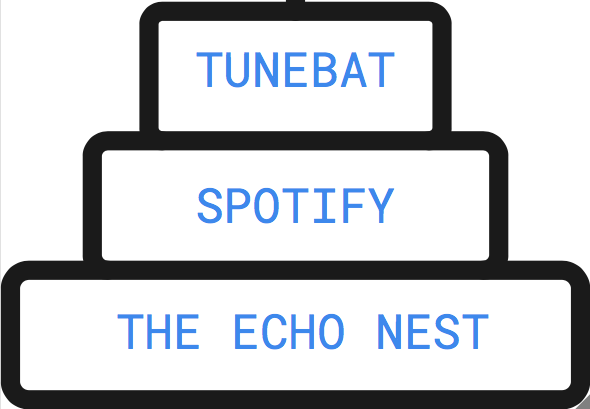
\includegraphics{./picturesDocu/dependencies.png}
\caption{selfcreated graphical description of platform dependencies}
\end{figure}

It is not clear weather both platforms can be compared. The intension to
compare the platforms did come up, because it would be better to have
some more information about the songs regarding the emotion or the
genre. So Tunebat provides those values. But first one should compare
the given songs and find out if Tunebat could be used for such a
comparison.

What also should be mentioned before is that listening to those songs
did get quite the same answers regarding the variables, besides the
Justin Timberlake song. Our assumption was that the data in the MDS
dataset for Justin Timberlake is not correct.

\begin{Shaded}
\begin{Highlighting}[]
\CommentTok{# create radar chart from tunebat.com }
\CommentTok{# loudness <- loudness}
\CommentTok{# tempo <- BPM}
\CommentTok{# mode <- KEY}
\CommentTok{# key <- KEY}
\NormalTok{compareFrame <-}\StringTok{ }\KeywordTok{data.frame}\NormalTok{(}\KeywordTok{rbind}\NormalTok{(}
  \DataTypeTok{beyonce =} \KeywordTok{c}\NormalTok{( }\StringTok{'loudness '}\NormalTok{ =}\StringTok{ }\OperatorTok{-}\DecValTok{5}\NormalTok{, }\StringTok{'tempo'}\NormalTok{ =}\StringTok{ }\DecValTok{97}\NormalTok{,}\StringTok{'mode'}\NormalTok{ =}\StringTok{ }\DecValTok{0}\NormalTok{, }\StringTok{'key'}\NormalTok{ =}\StringTok{ }\DecValTok{11}\NormalTok{),}
  \DataTypeTok{justin =} \KeywordTok{c}\NormalTok{( }\StringTok{'loudness '}\NormalTok{ =}\StringTok{ }\OperatorTok{-}\DecValTok{5}\NormalTok{, }\StringTok{'tempo'}\NormalTok{ =}\StringTok{ }\DecValTok{76}\NormalTok{, }\StringTok{'mode'}\NormalTok{ =}\StringTok{ }\DecValTok{1}\NormalTok{, }\StringTok{'key'}\NormalTok{ =}\StringTok{ }\DecValTok{7}\NormalTok{),}
  \DataTypeTok{kanye =} \KeywordTok{c}\NormalTok{(}\StringTok{'loudness '}\NormalTok{ =}\StringTok{ }\OperatorTok{-}\DecValTok{5}\NormalTok{, }\StringTok{'tempo'}\NormalTok{ =}\StringTok{ }\DecValTok{106}\NormalTok{, }\StringTok{'mode'}\NormalTok{ =}\StringTok{ }\DecValTok{1}\NormalTok{,}\StringTok{'key'}\NormalTok{ =}\StringTok{ }\DecValTok{9}\NormalTok{),}
  \DataTypeTok{madonna =} \KeywordTok{c}\NormalTok{( }\StringTok{'loudness '}\NormalTok{ =}\StringTok{ }\OperatorTok{-}\DecValTok{8}\NormalTok{, }\StringTok{'tempo'}\NormalTok{ =}\StringTok{ }\DecValTok{130}\NormalTok{, }\StringTok{'mode'}\NormalTok{ =}\StringTok{ }\DecValTok{0}\NormalTok{,}\StringTok{'key'}\NormalTok{ =}\StringTok{ }\DecValTok{4}\NormalTok{),}
  \DataTypeTok{bruno =} \KeywordTok{c}\NormalTok{( }\StringTok{'loudness '}\NormalTok{ =}\StringTok{ }\OperatorTok{-}\DecValTok{6}\NormalTok{, }\StringTok{'tempo'}\NormalTok{ =}\StringTok{ }\DecValTok{104}\NormalTok{, }\StringTok{'mode'}\NormalTok{ =}\StringTok{ }\DecValTok{1}\NormalTok{, }\StringTok{'key'}\NormalTok{ =}\StringTok{ }\DecValTok{10}\NormalTok{)}
\NormalTok{))}

\NormalTok{\{}
\CommentTok{# plot the two radarcharts together in one plot}
\KeywordTok{par}\NormalTok{(}\DataTypeTok{mfrow =} \KeywordTok{c}\NormalTok{(}\DecValTok{1}\NormalTok{,}\DecValTok{2}\NormalTok{))}
\KeywordTok{radar}\NormalTok{(data,}\DataTypeTok{x=}\OperatorTok{-}\FloatTok{2.2}\NormalTok{, }\DataTypeTok{y =} \OperatorTok{-}\FloatTok{1.2}\NormalTok{)}
\KeywordTok{radar}\NormalTok{(compareFrame,}\DataTypeTok{x=}\OperatorTok{-}\FloatTok{2.2}\NormalTok{,  }\DataTypeTok{y =} \OperatorTok{-}\FloatTok{1.2}\NormalTok{)}
\KeywordTok{title}\NormalTok{(}\StringTok{'Comparison between MSD and Tunebat'}\NormalTok{, }\DataTypeTok{outer =} \OtherTok{TRUE}\NormalTok{, }\DataTypeTok{line =} \OperatorTok{-}\DecValTok{1}\NormalTok{)}
\KeywordTok{par}\NormalTok{(}\DataTypeTok{mfrow =} \KeywordTok{c}\NormalTok{(}\DecValTok{1}\NormalTok{,}\DecValTok{1}\NormalTok{))}
\NormalTok{\}}
\end{Highlighting}
\end{Shaded}

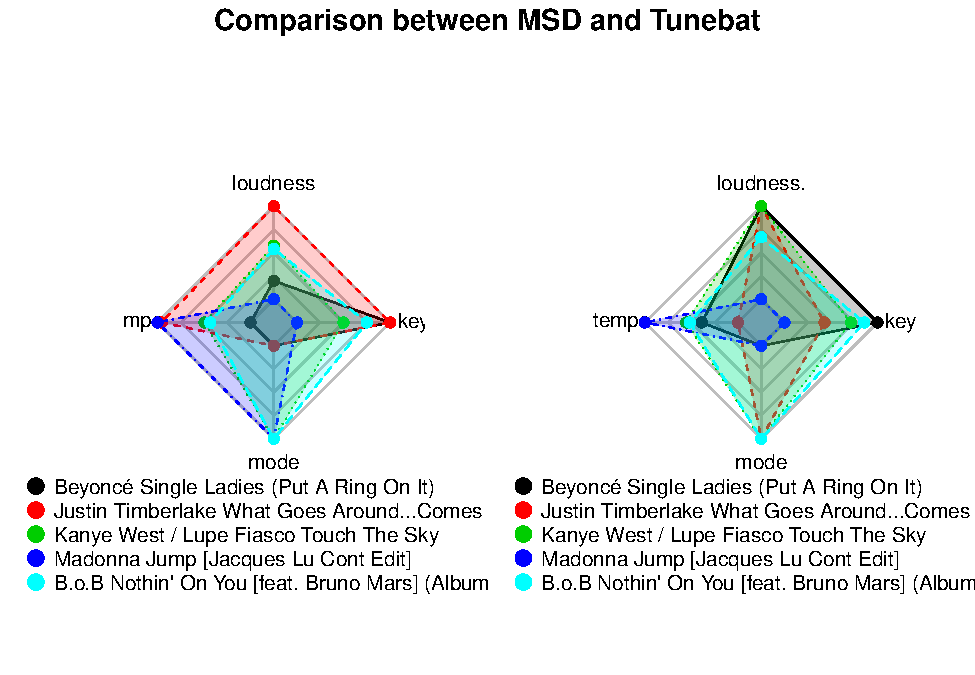
\includegraphics{Project2_files/figure-latex/compareTunebat-1.pdf}

When comparing the two platforms it seems that the songs do not have any
similarities. This could be described through the song data.

Artists do create songs, but sometimes there are many versions of those
songs and it is hard to find the right one to compare them. Even if the
songname is the same it could be modifyed. So in this case that
explanation could fit, or simply that either the first or the second
dataset is falsified. Since both platforms are not comparable the data
from the second platform, Tunebat could be rejected. We will restrict
ourseves only to the data provided from MSD.

\subsubsection{Detailed comparrison}\label{detailed-comparrison}

Since it is not possible to take a closer look on dancability or
hapiness of a song, provided by tunebat, we restricted ourselves to the
MSD dataset and the provided information in that data. However this
information can be be approached through variables in the MSD dataset.
Our focus will be on `artist\_familiarity', `artist\_hotnesss', `key'
and `tempo'.

The new strategie, since it is hard to compare the variables is, to take
the prefered songs and the variables and to average them for further
predictions and comparisons. First it would be nice to have a Barplot
for each prefered song and each taken variable, as mentioned before.

\begin{Shaded}
\begin{Highlighting}[]
\CommentTok{# Overall Barplot function for any dataframe  }
\NormalTok{crateBarplotOfFrame <-}\StringTok{ }\ControlFlowTok{function}\NormalTok{(x,y, NameP, }\DataTypeTok{rownames =} \OtherTok{FALSE}\NormalTok{)\{}
  \KeywordTok{barplot}\NormalTok{(x[,y], }\DataTypeTok{main =}\NormalTok{ y, }\DataTypeTok{col =} \DecValTok{1}\OperatorTok{:}\KeywordTok{dim}\NormalTok{(x)[}\DecValTok{1}\NormalTok{], }\DataTypeTok{horiz =} \OtherTok{TRUE}\NormalTok{, }\DataTypeTok{names.arg=} \ControlFlowTok{if}\NormalTok{(rownames)\{}\KeywordTok{row.names}\NormalTok{(NameP)\}}\ControlFlowTok{else}\NormalTok{\{}\KeywordTok{names}\NormalTok{(NameP)\}, }\DataTypeTok{cex.names=}\FloatTok{0.8}\NormalTok{, }\DataTypeTok{las =} \DecValTok{1}\NormalTok{)}
\NormalTok{\}}

\NormalTok{\{}
\CommentTok{# Bar plots for MSD}
\KeywordTok{par}\NormalTok{(}\DataTypeTok{mfrow =}\KeywordTok{c}\NormalTok{(}\DecValTok{2}\NormalTok{,}\DecValTok{2}\NormalTok{))}
\KeywordTok{crateBarplotOfFrame}\NormalTok{(Meta_song,}\StringTok{'artist_familiarity'}\NormalTok{, SubPaths)}
\KeywordTok{crateBarplotOfFrame}\NormalTok{(Meta_song,}\StringTok{'artist_hotttnesss'}\NormalTok{, SubPaths)}
\KeywordTok{crateBarplotOfFrame}\NormalTok{(Analyze_song,}\StringTok{'tempo'}\NormalTok{, SubPaths)}
\KeywordTok{crateBarplotOfFrame}\NormalTok{(Analyze_song,}\StringTok{'key'}\NormalTok{, SubPaths)}
\KeywordTok{title}\NormalTok{(}\StringTok{'Barplots for choosen songs and variables'}\NormalTok{, }\DataTypeTok{outer =} \OtherTok{TRUE}\NormalTok{, }\DataTypeTok{line =} \OperatorTok{-}\StringTok{ }\DecValTok{15}\NormalTok{)}
\KeywordTok{par}\NormalTok{(}\DataTypeTok{mfrow =}\KeywordTok{c}\NormalTok{(}\DecValTok{1}\NormalTok{,}\DecValTok{1}\NormalTok{))}
\NormalTok{\}}
\end{Highlighting}
\end{Shaded}

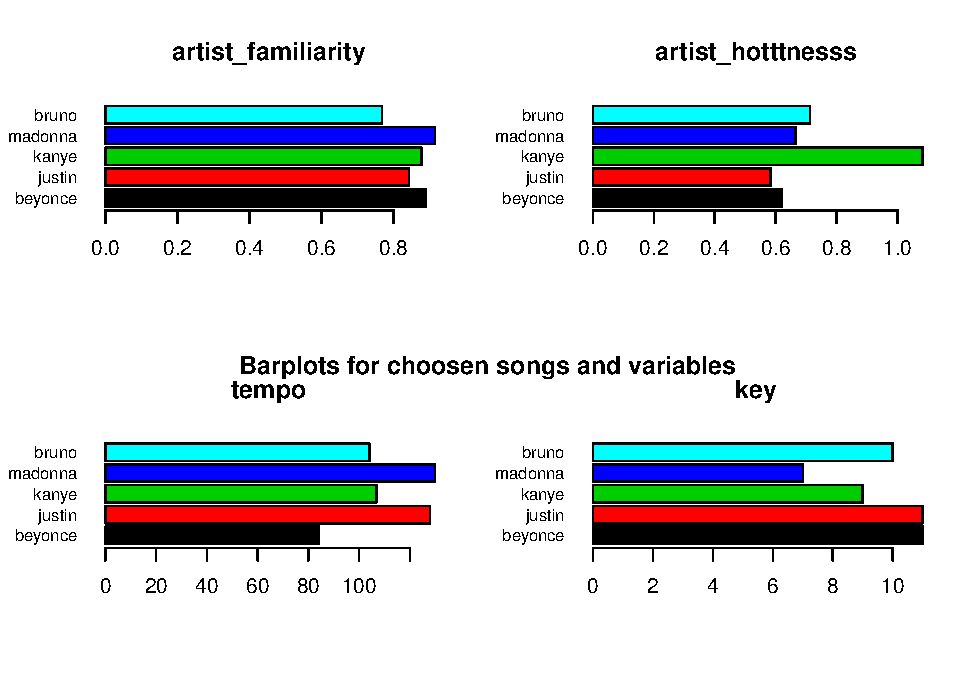
\includegraphics{Project2_files/figure-latex/MSDBarplots-1.pdf}

Now one can see directly the differences between each variable and each
song. The given artist familiarity is quite similar. All artists are
quite popular in 2010. This could also be a reason why one of our group
members picked those songs. During that time he probably did go to a lot
of discotheks and was probably listening a lot to this music.

The hotness however does vary a lot especially for kanye west which
outrages all other artist. This could be attributable through a new
single that he maybe published in this year and therefore got all the
buzz.

The tempo does also vary quite a lot and therefore it is hard to tell
which tempo the listener prefers. He probably likes fast and happy songs
more but also there is a more slower song. So he does listen to maybe
sad music too. People listen to music to project their feelings on to
it. This preferation could be used to profile the listener too. One
could say that the listener mostly is a happy person but sometimes tends
to be sad too.

The key in this case tends to be more in the higher sphere, what
actually regards to the time the music was produced in. Since the 21th
century music tend to be produced more Louder and mostly in G, which is
a higher key.

\subsubsection{Spotify recomendation
analysis}\label{spotify-recomendation-analysis}

Since we did not wanted to pick some random musicfiles, we created a
playlist on spotify, which contained exactly the preferation of one of
our groups member. Luckily Spotify provides some recomendation based on
the actual playlist. We used this recomendation to get more interesting
results for research purposes. However the used dataset did not provide
all recomended music from spotify and we had to refresh the
recomendations a couple of times to get the songs, which MSD contains.

Finaly we found three different songs, that MSD provides too.

\begin{itemize}
\tightlist
\item
  Lady GaGa - Poker Face
\item
  Sean Paul - Baby Boy {[}feat. Beyonce{]}
\item
  Shakira Featuring Wyclef - Jean Hips Don't Lie (featuring Wyclef Jean)
\end{itemize}

The goal now was to create an average of the prefered songs and
variables and plot it together with the recomended songs.

\begin{Shaded}
\begin{Highlighting}[]
\CommentTok{# create array with found Ids in beforehand containing prefered songs}
\NormalTok{TrackIDs <-}\StringTok{ }\KeywordTok{array}\NormalTok{(}\KeywordTok{c}\NormalTok{(}\StringTok{'TRAZWGK128F93141E3'}\NormalTok{,}\StringTok{'TRBDOVF128E0795641'}\NormalTok{,}\StringTok{'TRAAKDG128F42A0ECB'}\NormalTok{))}

\CommentTok{# find automaticaly all paths with names of trackIDs}
\NormalTok{SubPaths <-}\StringTok{ }\KeywordTok{lapply}\NormalTok{(TrackIDs,}\ControlFlowTok{function}\NormalTok{(x)\{}
  \KeywordTok{list.files}\NormalTok{(pathToSet, x, }\DataTypeTok{recursive=}\OtherTok{TRUE}\NormalTok{, }\DataTypeTok{full.names=}\OtherTok{TRUE}\NormalTok{, }\DataTypeTok{include.dirs=}\OtherTok{TRUE}\NormalTok{)}
\NormalTok{\})}

\CommentTok{# beautify the dataset }
\NormalTok{SubPaths <-}\StringTok{ }\KeywordTok{data.frame}\NormalTok{(}\DataTypeTok{SubPaths =} \KeywordTok{t}\NormalTok{(}\KeywordTok{unlist}\NormalTok{(SubPaths)))}
\KeywordTok{names}\NormalTok{(SubPaths) <-}\StringTok{ }\KeywordTok{c}\NormalTok{(}\StringTok{'Lady Gaga'}\NormalTok{, }\StringTok{'Sean Paul'}\NormalTok{, }\StringTok{'Shakira'}\NormalTok{)}

\CommentTok{# data from analysis song}
\NormalTok{R_Analyze_song <-}\StringTok{ }\KeywordTok{apply}\NormalTok{(SubPaths,}\DecValTok{2}\NormalTok{,}\ControlFlowTok{function}\NormalTok{(x)\{}
  \KeywordTok{h5read}\NormalTok{(x,}\StringTok{"/analysis/songs"}\NormalTok{)}
\NormalTok{\})}
\NormalTok{R_Analyze_song <-}\StringTok{ }\KeywordTok{do.call}\NormalTok{(rbind, R_Analyze_song)}

\CommentTok{# data from meta song}
\NormalTok{R_Meta_song <-}\StringTok{ }\KeywordTok{apply}\NormalTok{(SubPaths,}\DecValTok{2}\NormalTok{,}\ControlFlowTok{function}\NormalTok{(x)\{}
  \KeywordTok{h5read}\NormalTok{(x,}\StringTok{"/metadata/songs"}\NormalTok{)}
\NormalTok{\})}
\NormalTok{R_Meta_song <-}\StringTok{ }\KeywordTok{do.call}\NormalTok{(rbind, R_Meta_song)}

\CommentTok{# cretae better comparrison for songs}
\NormalTok{P_songs <-}\StringTok{ }\KeywordTok{cbind}\NormalTok{(}\StringTok{'artist_familiarity'}\NormalTok{ =}\StringTok{  }\KeywordTok{mean}\NormalTok{(Meta_song}\OperatorTok{$}\NormalTok{artist_familiarity), }\StringTok{'artist_hotttnesss'}\NormalTok{ =}\StringTok{ }\KeywordTok{mean}\NormalTok{(Meta_song}\OperatorTok{$}\NormalTok{artist_hotttnesss), }\StringTok{'tempo'}\NormalTok{ =}\StringTok{ }\KeywordTok{mean}\NormalTok{(Analyze_song}\OperatorTok{$}\NormalTok{tempo),  }\StringTok{'key'}\NormalTok{ =}\StringTok{ }\KeywordTok{mean}\NormalTok{(Analyze_song}\OperatorTok{$}\NormalTok{key))}
\NormalTok{R_songs <-}\StringTok{ }\KeywordTok{cbind}\NormalTok{(}\StringTok{'artist_familiarity'}\NormalTok{ =}\StringTok{ }\NormalTok{R_Meta_song}\OperatorTok{$}\NormalTok{artist_familiarity, }\StringTok{'artist_hotttnesss'}\NormalTok{ =}\StringTok{ }\NormalTok{R_Meta_song}\OperatorTok{$}\NormalTok{artist_hotttnesss, }\StringTok{'tempo'}\NormalTok{ =}\StringTok{ }\NormalTok{R_Analyze_song}\OperatorTok{$}\NormalTok{tempo, }\StringTok{'key'}\NormalTok{ =}\StringTok{ }\NormalTok{R_Analyze_song}\OperatorTok{$}\NormalTok{key)}

\NormalTok{MSD_R <-}\StringTok{ }\KeywordTok{data.frame}\NormalTok{(}\KeywordTok{rbind}\NormalTok{(P_songs,R_songs), }\DataTypeTok{row.names =} \KeywordTok{c}\NormalTok{(}\StringTok{"p_avg"}\NormalTok{,}\KeywordTok{row.names}\NormalTok{(R_Meta_song)[}\DecValTok{1}\OperatorTok{:}\DecValTok{3}\NormalTok{]))}

\NormalTok{\{}
\KeywordTok{par}\NormalTok{(}\DataTypeTok{mfrow =} \KeywordTok{c}\NormalTok{(}\DecValTok{2}\NormalTok{,}\DecValTok{2}\NormalTok{))}
\KeywordTok{crateBarplotOfFrame}\NormalTok{(MSD_R,}\StringTok{'artist_familiarity'}\NormalTok{, MSD_R, }\OtherTok{TRUE}\NormalTok{)}
\KeywordTok{crateBarplotOfFrame}\NormalTok{(MSD_R,}\StringTok{'artist_hotttnesss'}\NormalTok{, MSD_R, }\OtherTok{TRUE}\NormalTok{)}
\KeywordTok{crateBarplotOfFrame}\NormalTok{(MSD_R,}\StringTok{'tempo'}\NormalTok{, MSD_R, }\OtherTok{TRUE}\NormalTok{)}
\KeywordTok{crateBarplotOfFrame}\NormalTok{(MSD_R,}\StringTok{'key'}\NormalTok{,MSD_R, }\OtherTok{TRUE}\NormalTok{)}
\KeywordTok{title}\NormalTok{(}\DataTypeTok{main =} \StringTok{'Spotify recomended titles with average of prefered Songs'}\NormalTok{, }\DataTypeTok{outer =} \OtherTok{TRUE}\NormalTok{, }\DataTypeTok{line =} \OperatorTok{-}\DecValTok{15}\NormalTok{)}
\KeywordTok{par}\NormalTok{(}\DataTypeTok{mfrow =} \KeywordTok{c}\NormalTok{(}\DecValTok{1}\NormalTok{,}\DecValTok{1}\NormalTok{))}
\NormalTok{\}}
\end{Highlighting}
\end{Shaded}

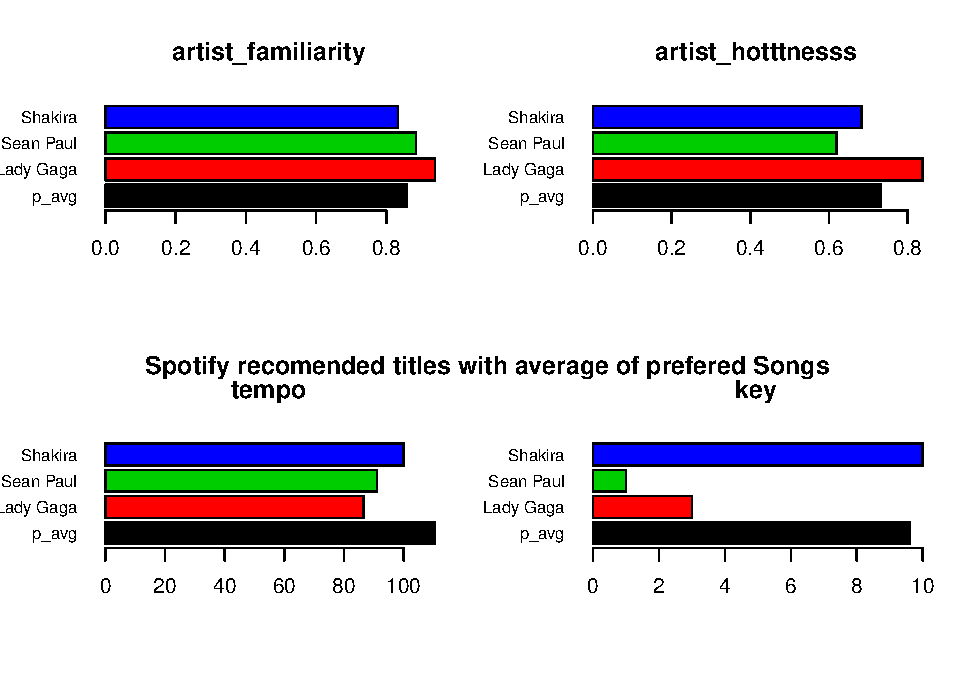
\includegraphics{Project2_files/figure-latex/RecomendBoxplots-1.pdf}

Based on the results above one can do a very good prediction either to
recomend or not to recomend those songs.

Starting with the familiarity it is obvious that all artists are quite
popular but `Sean Paul' and `Shakira' tend to be closer to the average
then `Lady GaGa'. Therefore one would recomend either `Sean Paul' or
`Shakira'. But based on only one variable it is hard to tell weather the
result is a confident one.

So taking a look on hotness one can see that `Sean Paul' and `Shakira'
are not as hot as `Lady GaGa'. This could have many reasons. One could
be regarding only this artists and the particular song, that the songs
where released in `Sean Paul' 2003, `Shakira' 2006 and `Lady GaGa' 2008.
Therefore Lady GaGa has the most hotness and a very big buzz. Also one
could asume, that `Lady GaGa' did produce a new song and released it
around 2010. The prediction for this variable would be `Shakira'.

The recomended songs tend to be more slow then the prefered ones. First
one could assume that the songs are slower and therefore sadlier. This
However can not be seen through a quantitative analysis and needs to be
prooved either through a qualitative analysis or even through NLP and
the written text. One could derive together with the text and the tempo
the emotion of the song. looking at this variable one would also prefer
`Shakira'.

because keys are distinct, there is no proper average in the sence of an
actual mathematical average. The calculated average needs to be roundet
up or down. In this case the average stays the same but with a remark to
the actual one. So taking a closer look at this variable one would
recomend to take `Shakira' too.

To sum up the variables and make a first prediction. `Shakira' and `Sean
Paul' tend to be very suitable for the listener and would be probably
recomended. One should take `Shakira' and'Sean Paul' first and `Lady
GaGa' second to recomd it to the listener. To be more accurate about
this prediction, one should also assume to make a boxplot to see how
confident the results are. This can be seen in the plot below.

\begin{Shaded}
\begin{Highlighting}[]
\NormalTok{crateBoxplotOfFrame <-}\StringTok{ }\ControlFlowTok{function}\NormalTok{(x,y,xDerive, }\DataTypeTok{limStart =} \DecValTok{0}\NormalTok{, }\DataTypeTok{limEnd =} \DecValTok{1}\NormalTok{)\{}
  \KeywordTok{boxplot}\NormalTok{(x[,y], }\DataTypeTok{las =} \DecValTok{2}\NormalTok{ , }\DataTypeTok{main=}\NormalTok{ y, }\DataTypeTok{ylim=}\KeywordTok{c}\NormalTok{(limStart,limEnd))}
\KeywordTok{abline}\NormalTok{(}\DataTypeTok{h=}\NormalTok{xDerive[,y], }\DataTypeTok{col =}\DecValTok{2}\OperatorTok{:}\NormalTok{(}\KeywordTok{dim}\NormalTok{(xDerive)[}\DecValTok{1}\NormalTok{]}\OperatorTok{+}\DecValTok{1}\NormalTok{))}
\KeywordTok{axis}\NormalTok{(}\DecValTok{1}\NormalTok{, }\DataTypeTok{labels=}\KeywordTok{c}\NormalTok{(}\StringTok{"playlist"}\NormalTok{), }\DataTypeTok{at=}\DecValTok{1}\NormalTok{, }\DataTypeTok{las=}\DecValTok{1}\NormalTok{)}
\NormalTok{\}}

\NormalTok{\{}
\KeywordTok{layout}\NormalTok{(}\KeywordTok{matrix}\NormalTok{(}\KeywordTok{c}\NormalTok{(}\DecValTok{1}\NormalTok{,}\DecValTok{2}\NormalTok{,}\DecValTok{1}\NormalTok{,}\DecValTok{3}\NormalTok{),}\DecValTok{2}\NormalTok{,}\DecValTok{2}\NormalTok{,}\DataTypeTok{byrow =} \OtherTok{TRUE}\NormalTok{))}
\KeywordTok{crateBoxplotOfFrame}\NormalTok{(Meta_song,}\StringTok{'artist_familiarity'}\NormalTok{,R_Meta_song,}\FloatTok{0.7}\NormalTok{,}\DecValTok{1}\NormalTok{)}
\KeywordTok{crateBoxplotOfFrame}\NormalTok{(Meta_song,}\StringTok{'artist_hotttnesss'}\NormalTok{,R_Meta_song,}\FloatTok{0.5}\NormalTok{,}\FloatTok{0.9}\NormalTok{)}
\KeywordTok{crateBoxplotOfFrame}\NormalTok{(Analyze_song,}\StringTok{'tempo'}\NormalTok{,R_Analyze_song,}\DecValTok{80}\NormalTok{,}\DecValTok{130}\NormalTok{)}
\KeywordTok{title}\NormalTok{(}\DataTypeTok{main =} \StringTok{'boxplots for confidence'}\NormalTok{, }\DataTypeTok{outer =} \OtherTok{TRUE}\NormalTok{, }\DataTypeTok{line =} \OperatorTok{-}\DecValTok{1}\NormalTok{)}
\KeywordTok{par}\NormalTok{(}\DataTypeTok{mfrow =} \KeywordTok{c}\NormalTok{(}\DecValTok{1}\NormalTok{,}\DecValTok{1}\NormalTok{))}
\NormalTok{\}}
\end{Highlighting}
\end{Shaded}

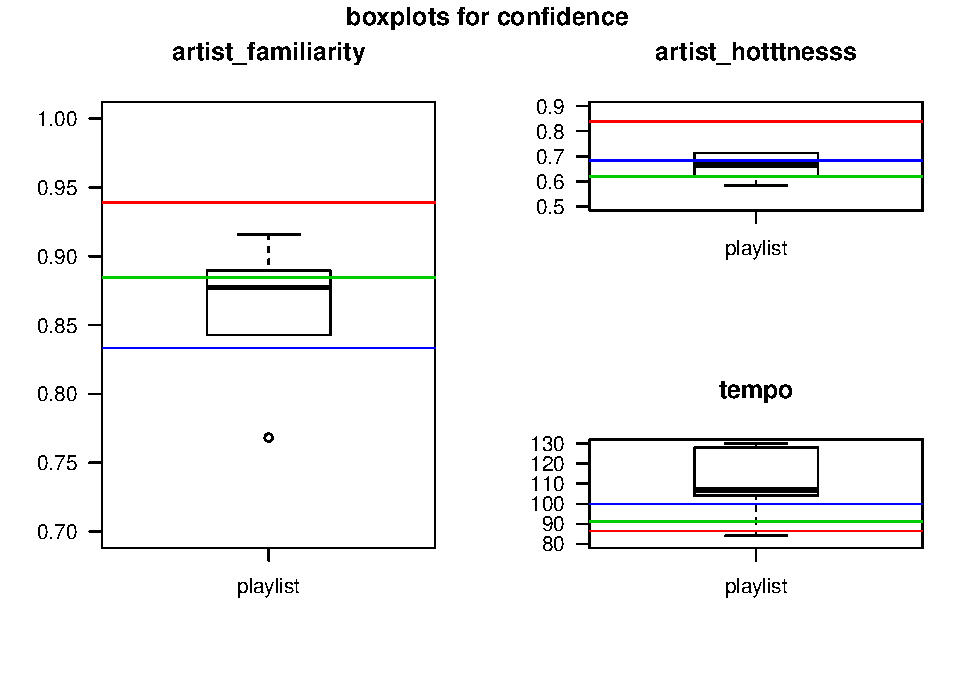
\includegraphics{Project2_files/figure-latex/Boxplot-1.pdf}

Since key is distinct, it was not ploted as a boxplot. So looking at the
given boxplots one can see, that the assumptions for familiarity do not
tend to be between `Shakira' and `Sean Paul' but only `Sean Paul'.
Whereas by looking at the hotness both would be recomended. Finally the
tempo, where all the recomendations seemed to be outliers, all of the
songs would be recomended.

Summing up the boxplots above one will see that regarding to the
barplots one can not fully understand the data but combined with the
boxplots it gets more clear and the dataset is wrangled up more. The
final recomendation according to the data would be `Shakira' first,
because she tends to fit more the average then the others, `Sean Paul'
second and `Lady GaGa' last.

But a proper recomendation based on this variables is still verry hard
and we are not sure how confident this recomendation is. Therefore we
would like to use some Data mining methods like PCA on timbre as well as
the pitch.

\subsubsection{PCA analysis}\label{pca-analysis}

The plot below shows the provided PCA for timbre in each song. Here we
used only PC1 and PC2, since both do map the most variaty of the data.
We hope for a good clustering that either could proove our assumption or
give us some more detailes about the recomendation of those recomended
songs.

\begin{Shaded}
\begin{Highlighting}[]
\NormalTok{#############################}

\CommentTok{# averaged timbre of prefered songs}
\NormalTok{mean_timbre <-}\StringTok{ }\KeywordTok{t}\NormalTok{(}\KeywordTok{sapply}\NormalTok{(track_timbre, }\ControlFlowTok{function}\NormalTok{(x)\{}\KeywordTok{apply}\NormalTok{(x,}\DecValTok{1}\NormalTok{,mean)\} ))}

\CommentTok{# timbre recommended song}
\NormalTok{R_track_timbre <-}\StringTok{ }\KeywordTok{apply}\NormalTok{(SubPaths,}\DecValTok{2}\NormalTok{,}\ControlFlowTok{function}\NormalTok{(x)\{}
  \KeywordTok{h5read}\NormalTok{(x,}\StringTok{"/analysis/segments_timbre"}\NormalTok{)}
\NormalTok{\})}

\CommentTok{# recomended songs averaged}
\NormalTok{R_mean_timbre <-}\StringTok{ }\KeywordTok{t}\NormalTok{(}\KeywordTok{sapply}\NormalTok{(R_track_timbre, }\ControlFlowTok{function}\NormalTok{(x)\{}\KeywordTok{apply}\NormalTok{(x,}\DecValTok{1}\NormalTok{,mean)\} ))}

\CommentTok{# plot of recomended timbre and prefered songs timbre}
\CommentTok{#par(mar=c(5,5,4,2))}
\KeywordTok{plot}\NormalTok{(mean_timbre[,}\DecValTok{1}\NormalTok{], mean_timbre[,}\DecValTok{2}\NormalTok{], }\DataTypeTok{ylim=}\KeywordTok{c}\NormalTok{(}\OperatorTok{-}\DecValTok{50}\NormalTok{,}\DecValTok{50}\NormalTok{), }\DataTypeTok{xlim=}\KeywordTok{c}\NormalTok{(}\DecValTok{35}\NormalTok{,}\DecValTok{50}\NormalTok{), }\DataTypeTok{xlab =} \StringTok{'timbre PC1 =  average loudness of the segments averaged'}\NormalTok{, }\DataTypeTok{ylab =} \StringTok{'timbre PC2 = brightness'}\NormalTok{)}
\KeywordTok{text}\NormalTok{(mean_timbre[,}\DecValTok{1}\NormalTok{], mean_timbre[,}\DecValTok{2}\NormalTok{], }\DataTypeTok{labels=}\KeywordTok{row.names}\NormalTok{(mean_timbre), }\DataTypeTok{cex=} \FloatTok{0.7}\NormalTok{, }\DataTypeTok{pos=}\DecValTok{3}\NormalTok{)}
\KeywordTok{points}\NormalTok{(R_mean_timbre[,}\DecValTok{1}\NormalTok{], R_mean_timbre[,}\DecValTok{2}\NormalTok{], }\DataTypeTok{pch=}\DecValTok{21}\NormalTok{,  }\DataTypeTok{bg=}\StringTok{"lightgreen"}\NormalTok{)}
\KeywordTok{text}\NormalTok{(R_mean_timbre[,}\DecValTok{1}\NormalTok{], R_mean_timbre[,}\DecValTok{2}\NormalTok{], }\DataTypeTok{labels=}\KeywordTok{row.names}\NormalTok{(R_mean_timbre), }\DataTypeTok{cex=} \FloatTok{0.7}\NormalTok{, }\DataTypeTok{pos=}\DecValTok{3}\NormalTok{)}
\KeywordTok{title}\NormalTok{(}\DataTypeTok{main =} \StringTok{'PCA timbre for recomended and preferden Songs'}\NormalTok{)}
\end{Highlighting}
\end{Shaded}

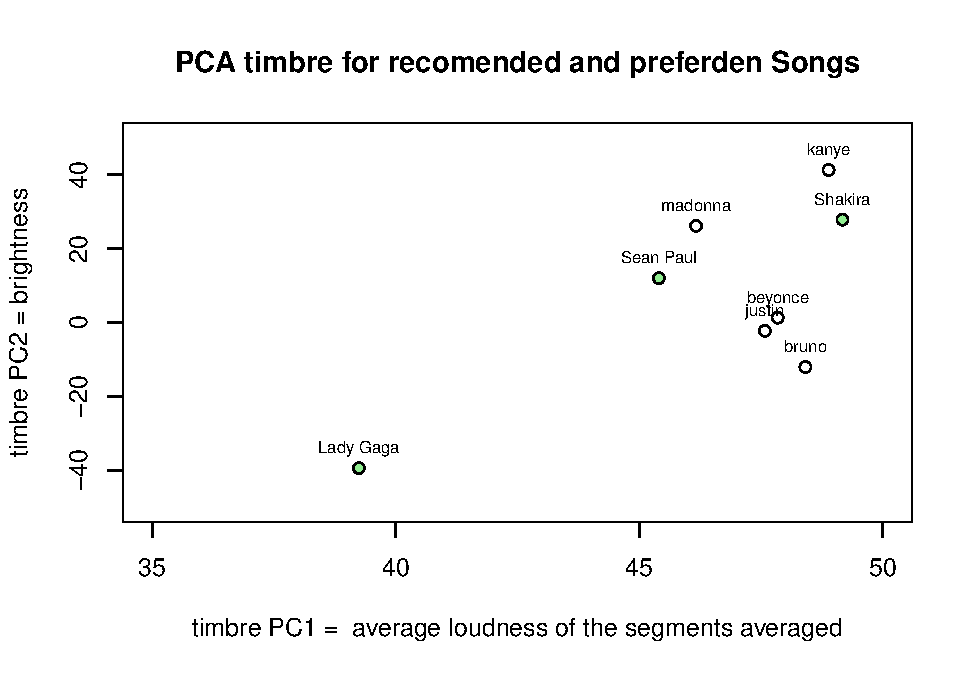
\includegraphics{Project2_files/figure-latex/PCATimbre-1.pdf}

Looking at the plot one can recognize four different groups. But three
of them tend to be more similar then the fourth. Since timbre gives a
good overview of the whole dataset and the musical mood. It is quite
good to use, when trying to recomend a song or to find similar songs in
the dataset. Even if the timbre fits quite well it is hard to read and
understand, because it consists out of 12 x N observations and the 12
observations describe Princiopal Components. Nevertheless for prooving
our recomendation we take timbre as well as the pitch , where we
calculate the Principal component and plot the first two too.

\begin{Shaded}
\begin{Highlighting}[]
\CommentTok{# averaged pitch of prefered songs}
\NormalTok{mean_pitch <-}\StringTok{ }\OtherTok{NULL}
\ControlFlowTok{for}\NormalTok{(i }\ControlFlowTok{in} \KeywordTok{names}\NormalTok{(track_pitch))\{}
  \CommentTok{#pca}
\NormalTok{  pr <-}\KeywordTok{prcomp}\NormalTok{(}\KeywordTok{t}\NormalTok{(track_pitch[[i]]),}\DataTypeTok{scale=}\OtherTok{TRUE}\NormalTok{)}
  \CommentTok{#mean from pca}
\NormalTok{  res <-}\StringTok{ }\KeywordTok{apply}\NormalTok{(}\KeywordTok{t}\NormalTok{(pr}\OperatorTok{$}\NormalTok{x),}\DecValTok{1}\NormalTok{,mean)}
\NormalTok{  mean_pitch <-}\StringTok{ }\KeywordTok{rbind}\NormalTok{(mean_pitch,res)}
\NormalTok{\}}
\KeywordTok{row.names}\NormalTok{(mean_pitch) <-}\StringTok{ }\KeywordTok{names}\NormalTok{(track_pitch)}

\CommentTok{# pitch recommended songs}
\NormalTok{R_track_pitch <-}\StringTok{ }\KeywordTok{apply}\NormalTok{(SubPaths,}\DecValTok{2}\NormalTok{,}\ControlFlowTok{function}\NormalTok{(x)\{}
  \KeywordTok{h5read}\NormalTok{(x,}\StringTok{"/analysis/segments_pitches"}\NormalTok{)}
\NormalTok{\})}

\CommentTok{# averaged pitch of recomended songs}
\NormalTok{R_mean_pitch <-}\StringTok{ }\OtherTok{NULL}
\ControlFlowTok{for}\NormalTok{(i }\ControlFlowTok{in} \KeywordTok{names}\NormalTok{(R_track_pitch))\{}
  \CommentTok{#pca}
\NormalTok{  pr <-}\KeywordTok{prcomp}\NormalTok{(}\KeywordTok{t}\NormalTok{(R_track_pitch[[i]]),}\DataTypeTok{scale=}\OtherTok{TRUE}\NormalTok{)}
  \CommentTok{#mean from pca}
\NormalTok{  res <-}\StringTok{ }\KeywordTok{apply}\NormalTok{(}\KeywordTok{t}\NormalTok{(pr}\OperatorTok{$}\NormalTok{x),}\DecValTok{1}\NormalTok{,mean)}
\NormalTok{  R_mean_pitch <-}\StringTok{ }\KeywordTok{rbind}\NormalTok{(R_mean_pitch,res)}
\NormalTok{\}}
\KeywordTok{row.names}\NormalTok{(R_mean_pitch) <-}\StringTok{ }\KeywordTok{names}\NormalTok{(R_track_pitch)}

\CommentTok{# plot of recomended pitch and prefered songs pitch}
\KeywordTok{par}\NormalTok{(}\DataTypeTok{mar=}\KeywordTok{c}\NormalTok{(}\DecValTok{5}\NormalTok{,}\DecValTok{6}\NormalTok{,}\DecValTok{3}\NormalTok{,}\DecValTok{2}\NormalTok{))}
\KeywordTok{plot}\NormalTok{(mean_pitch[,}\DecValTok{1}\NormalTok{], mean_pitch[,}\DecValTok{2}\NormalTok{], }\DataTypeTok{ylab=}\StringTok{""}\NormalTok{, }\DataTypeTok{xlab=}\StringTok{""}\NormalTok{ ,}\DataTypeTok{ylim =} \KeywordTok{c}\NormalTok{(}\OperatorTok{-}\FloatTok{6e-17}\NormalTok{,}\FloatTok{6e-17}\NormalTok{), }\DataTypeTok{xlim =} \KeywordTok{c}\NormalTok{(}\OperatorTok{-}\FloatTok{1.4e-16}\NormalTok{,}\FloatTok{5e-17}\NormalTok{))}
\KeywordTok{text}\NormalTok{(mean_pitch[,}\DecValTok{1}\NormalTok{], mean_pitch[,}\DecValTok{2}\NormalTok{], }\DataTypeTok{labels=}\KeywordTok{row.names}\NormalTok{(mean_pitch), }\DataTypeTok{cex=} \FloatTok{0.7}\NormalTok{, }\DataTypeTok{pos=}\DecValTok{3}\NormalTok{)}
\KeywordTok{title}\NormalTok{(}\DataTypeTok{xlab=}\StringTok{"pc1"}\NormalTok{,}\DataTypeTok{ylab=}\StringTok{"pc2"}\NormalTok{, }\DataTypeTok{main =} \StringTok{'PCA pitch for recomended and preferden Songs'}\NormalTok{)}
\KeywordTok{points}\NormalTok{(R_mean_pitch[,}\DecValTok{1}\NormalTok{], R_mean_pitch[,}\DecValTok{2}\NormalTok{], }\DataTypeTok{pch=}\DecValTok{21}\NormalTok{,  }\DataTypeTok{bg=}\StringTok{"lightgreen"}\NormalTok{)}
\KeywordTok{text}\NormalTok{(R_mean_pitch[,}\DecValTok{1}\NormalTok{], R_mean_pitch[,}\DecValTok{2}\NormalTok{], }\DataTypeTok{labels=}\KeywordTok{row.names}\NormalTok{(R_mean_pitch), }\DataTypeTok{cex=} \FloatTok{0.7}\NormalTok{, }\DataTypeTok{pos=}\DecValTok{3}\NormalTok{)}
\end{Highlighting}
\end{Shaded}

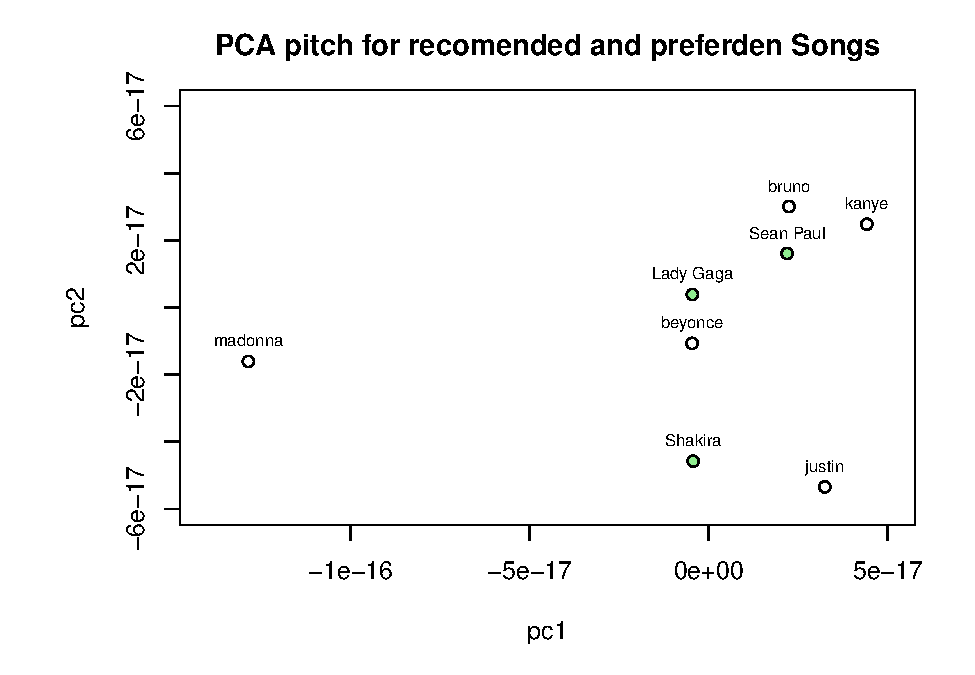
\includegraphics{Project2_files/figure-latex/PCAPitch-1.pdf}

The pitch PCA plot does provide even more groups as the tinbre PCA. Also
we can see, that both plots do have different results. When thinking
about the ploted result one can describe why the pitch does have a
different result then the timbre. The pitch does not give a good
overview about the dataset it only depends on the key values, whereas
timbre depends on the whole dataset.

To sum up both results, pitch does not fit for this kind of task. Timbre
PCA partly confirms the assumptions made in the sections before.

\section{Conclusion}\label{conclusion}

To Conclude the whole results, the listener should listen to the
recomended songs and make a qualitative analysis.

After doing so, the listener came to the exactly same result as
recomended. Therefore the assumptions made by the bar- and boxplots
where quite good and could be used for recomending more music to the
listener. Of course one could also use the timbre to recomend the music.
This assumption would be even better, since it recomended as well
`Shakira' as well as `Sean Paul', whereas the other assumption did a
grading.

We reached our goal, to find some similarities in prefered songs and
based on those recomend some other songs. Even though we used Spotify
for getting recomended songs, to be not picking randomly songs out of
the dataset that with a very high probability wont fit. Because mostly
the songs are from the 1940's, 1950's and 1960's.

\section{Sources and Footnotes}\label{sources-and-footnotes}

european map limits to draw with R:
\url{http://www.milanor.net/blog/maps-in-r-introduction-drawing-the-map-of-europe/}

comparison site: \url{https://tunebat.com/}

The H5 data explained:
\url{https://labrosa.ee.columbia.edu/millionsong/pages/example-track-description}

research:

\begin{itemize}
\tightlist
\item
  \url{https://www.musical-u.com/learn/rhythm-tips-for-identifying-music-genres-by-ear/}
\item
  \url{https://www.ncbi.nlm.nih.gov/pmc/articles/PMC4971092/}
\item
  \url{http://www.ee.columbia.edu/~dliang/files/FINAL.pdf}
\item
  \url{https://www.quora.com/How-does-Spotify-estimate-the-valence-of-a-song}
\item
  \url{https://techcrunch.com/2014/10/19/the-sonic-mad-scientists/}
\end{itemize}

on Key:

\begin{itemize}
\tightlist
\item
  \url{https://ledgernote.com/blog/lessons/musical-key-characteristics-emotions/}
\end{itemize}


\end{document}
